\documentclass[12pt,a4paper]{book}
\usepackage[french]{babel}
\usepackage[utf8]{inputenc}
\usepackage[T1]{fontenc}
\usepackage[a4paper, margin=2cm]{geometry}
\usepackage{amsmath, amsfonts, amssymb}
\usepackage{graphicx}
\usepackage{ragged2e}
\usepackage{setspace}
\usepackage[T1]{fontenc} %para escurecer a cor da fonte
\usepackage{lmodern}
\usepackage[mathcal]{eucal}
\usepackage{pdfpages}
\usepackage{latexsym}
\usepackage{minitoc}
\usepackage{pdftexcmds}
\usepackage{tikz}
\usepackage{bm}
\usepackage[all]{xy}
\usepackage{makeidx}
\usepackage{geometry}
\usepackage[multiple]{footmisc} %permite colocar virgulas entre footnotes
\usepackage{relsize} %permite aumentar o tamanho das integrais
\usepackage{pbox} %permite quebrar a linha numa tabela
\usepackage{paralist}
\usepackage[toc,page]{appendix}
\bibliographystyle{unsrt}

\newcommand{\ket}[1]{\ensuremath{|#1\rangle}\xspace} %mecanica quantica
\newcommand{\bra}[1]{\ensuremath{\langle #1|}\xspace} %mecanica quantica
\newcommand{\braket}[2]{\ensuremath{\langle #1|#2\rangle}\xspace} %mecanica quantica
\newcommand{\cent}[1]{$#1\,^{\circ}{\rm C}$} %degrees
% % % % % % % % % % % % % % % % % % % % % % % % % % % % % % % % % % % % %
\usepackage{fancyhdr} %para customizar o cabecalho
\pagestyle{fancy} %para customizar o cabecalho
\fancyhf{} %para customizar o cabecalho
\fancyhead[EL]{\nouppercase\leftmark} %para customizar o cabecalho
\fancyhead[OR]{\nouppercase\rightmark} %para customizar o cabecalho
\fancyhead[ER,OL]{\thepage} 

\usepackage{titlesec} %para centralizar o capitulo e o ti�tulo
\titleformat{\chapter}[display]%para centralizar o capitulo e o ti�tulo
{\normalfont\huge\bfseries\centering}{\chaptertitlename\ \thechapter}{20pt}{\Huge}%para centralizar o capitulo e o ti�tulo
\usepackage[shortcuts]{extdash} 
\begin{document}
\newenvironment{romanpages}
{\setcounter{page}{1}
	\renewcommand{\thepage}{\roman{page}}}
{\newpage\renewcommand{\thepage}{\arabic{page}}\setcounter{page}{1}}
\newcommand{\PRESn}{Dr Brigitte PEPIN-DONAT}
\newcommand{\PRESp}{CNRS, France}
\newcommand{\PRESq}{Président}

\newcommand{\INVAn}{Dr }
\newcommand{\INVAp}{xxxxxxx, Univ.}
\newcommand{\INVAq}{Invit\'e}
\newcommand{\RAPAn}{Dr Christophe RAYNAUD}
\newcommand{\RAPAp}{Universit\'e de Montpellier, France}
\newcommand{\RAPAq}{Rapporteur}
\newcommand{\RAPBn}{Dr Johannes GIERSCHNER}
\newcommand{\RAPBp}{IMDEA, Spain}
\newcommand{\RAPBq}{Rapporteur}

\newcommand{\EXAAn}{Dr Paul TOPHAM}
\newcommand{\EXAAp}{Aston University, UK}
\newcommand{\EXAAq}{Examinateur}

\newcommand{\EXABn}{Jury}
\newcommand{\EXABp}{UPPA}
\newcommand{\EXABq}{Examinateur}

\newcommand{\EXACn}{M.}
\newcommand{\EXACp}{xxxxxxxxxx}
\newcommand{\EXACq}{Examinateur}

\newcommand{\JURY}{
	\textbf{\large{\textbf{JURY}}}\\[\baselineskip]
	\begin{tabular}{l@{\protect\hspace{0.5cm}}l@{\protect\hspace{0.5cm}}l}
		%\textbf{\large{\textbf{Composition du jury :}}}
		\RAPAn &\RAPAp &\RAPAq\\
		\RAPBn &\RAPBp &\RAPBq\\
		\EXAAn &\EXAAp &\EXAAq\\
		%\EXABn &\EXABp &\EXABq\\
		\PRESn &\PRESp &\PRESq\\
		%\EXACn &\EXACp &\EXACq\\
		%\INVAn &\INVAp &\INVAq\\
	\end{tabular}
}

%\begin{minipage}[c]{15cm}
%\addtolength{\hoffset}{-0.5cm}
%\addtolength{\textwidth}{0.6cm} 
\thispagestyle{empty}
\newgeometry{left=2cm,bottom=2cm,right=2cm,top=1cm}
%\baselineskip=13pt
%\vspace*{-4cm}
\begin{center}

\includegraphics[height=2.2cm]{logo/uppa.png}
\end{center}
\begin{center}
	\hbox{\raisebox{0.4em}{\vrule depth 0pt height 1pt width 15cm}}\setlength{\baselineskip}{13pt}~\\
	{\Large{\textbf{THESES}}}\\[\baselineskip]
	préparée et présentée à \\[\baselineskip]
	L'UNIVERSIT\'E DE PAU ET DES PAYS DE L'ADOUR \\[\baselineskip]
	pour obtenir le grade de\\[\baselineskip]
		{\Large\textit{{\textbf{Docteur}}}}\\[\baselineskip]
	Spécialité : CHIMIE PHYSIQUE \\[\baselineskip]
	par\\[\baselineskip]
  	\baselineskip=20pt
	{\LARGE{\textbf{Patricia Guevara Level}}}\\
	Sujet de la thèse :\\
	\hbox{\raisebox{0.2em}{\vrule depth 0pt height 3.5pt width 17cm}}
	\setlength{\baselineskip}{4pt}
	\hbox{\raisebox{0.4em}{\vrule depth 0pt height 1pt width 17cm}}\setlength{\baselineskip}{10pt}~\\
	\vspace*{-5pt}
	{\Large\textbf{Title in English \\ \textit{Titre en français}}}~\\[\baselineskip]
	\hbox{\raisebox{0.4em}{\vrule depth 0pt height 1pt width 17cm}}~\\
	
	Directeur de Thèse: \textbf{Pr Didier B\'EGU\'E}\\[\baselineskip]
	Soutenue le  XXth, 2016\\[\baselineskip]
	devant la commission d'examen composée de :\\[\baselineskip]~\\[\baselineskip] 
	
	\JURY
\end{center}

% Nom profession Qualite du president du jury
\newcommand{\President}[3]{%
	\renewcommand{\PRESn}{#1}%
	\renewcommand{\PRESp}{#2}%
	\renewcommand{\PRESq}{#3}%
}

% Nom Profession Qualité de l'invité
\newcommand{\Invite}[3]{%
	\renewcommand{\INVAn}{#1}%
	\renewcommand{\INVAp}{#2}%
	\renewcommand{\INVAq}{#3}%
}

% Nom Profession Qualite d'un rapporteur A
\newcommand{\RapporteurA}[3]{%
	\renewcommand{\RAPAn}{#1}%
	\renewcommand{\RAPAp}{#2}%
	\renewcommand{\RAPAq}{#3}%
}
% Nom Profession Qualite d'un rapporteur B
\newcommand{\RapporteurB}[3]{%
	\renewcommand{\RAPBn}{#1}%
	\renewcommand{\RAPBp}{#2}%
	\renewcommand{\RAPBq}{#3}%
}

%Prenom Nom Qualite d'un examinateur A
\newcommand{\ExaminateurA}[3]{%
	\renewcommand{\EXAAn}{#1}%
	\renewcommand{\EXAAp}{#2}%
	\renewcommand{\EXAAq}{#3}%
}
%Prenom Nom Qualite d'un examinateur B
\newcommand{\ExaminateurB}[3]{%
	\renewcommand{\EXABn}{#1}%
	\renewcommand{\EXABp}{#2}%
	\renewcommand{\EXABq}{#3}%
}

%Prenom Nom Qualite d'un examinateur C
\newcommand{\ExaminateurC}[3]{%
	\renewcommand{\EXACn}{#1}%
	\renewcommand{\EXACp}{#2}%
	\renewcommand{\EXACq}{#3}%
}



% une page blanche (deuxième de couverture)

\newpage\thispagestyle{empty}\addtocounter{page}{-5}
\null\newpage\thispagestyle{empty}

%\newpage\thispagestyle{empty}
%~\newpage\thispagestyle{empty}
%\newpage

\setcounter{secnumdepth}{3}
\setcounter{tocdepth}{3}

\newenvironment{bottompar}{\par\vspace*{\fill}}{\clearpage}
\restoregeometry
\include{remerciements/remerciements}
\include{epigrafe/epigrafe}
\include{dedic/dedic}
\include{resumes/ingles}
\include{resumes/frances}
\renewcommand*\contentsname{Table of Contents} %troca o nome do sumario para o que quiser
\tableofcontents \thispagestyle{empty} 
\listoffigures \thispagestyle{empty} 
\listoftables \thispagestyle{empty}
\newpage
\include{abrev/abrev}
\newpage
\newgeometry{textwidth=16cm}
	\chapter*{Introduction}
	\minitoc
	\restoregeometry
	
	
	Les asphaltènes représentent une fraction du pétrole brut, définie sur la seule base de ses propriétés de solubilité. Ainsi, appartiennent à la famille des asphaltènes les composés chimiques du pétrole solubles dans les solvants aromatiques, tels que le toluène, mais insolubles dans les $n$-alcanes, tels le $n$-pentane ou le $n$-hexane. Cette définition, limitée à une unique propriété physique, laisse comprendre implicitement que la nature chimique des asphaltènes, c'est-à-dire leur composition aussi bien que le type et la forme des différentes structures moléculaires qui les constituent, reste inconnue. En somme, ces systèmes chimiques sont pareils à un puzzle dont on ne possèderait que l'emballage. Les propriétés macroscopiques -- la solubilité -- correspondent à l'image du puzzle présentée sur la boîte, mais le nombre de pièces, de même que leurs formes et la manière dont elles s'assemblent, nous sont inconnus. Tel est le défi auquel font face depuis de nombreuses années les chercheurs, aidés de leur palette de techniques expérimentales et de méthodes théoriques. L'enjeu est de taille, tant cette famille de composés pose de problèmes, aux divers stades de l'extraction, de la production et du raffinage du pétrole. Dans l'industrie pétrolière, le seul mot \og asphaltène \fg{} est invariablement associé aux phénomènes d'agrégation caractéristiques de ces systèmes, responsables entre autres de l'obstruction des pipelines. \\
	
	Au fil des années, diverses techniques de caractérisation ont permis de lever le voile sur une partie des propriétés chimiques de ces systèmes. Il est désormais admis que les asphaltènes sont formés d'un ensemble de structures moléculaires composées de noyaux aromatiques poly-condensés, ramifiés par des chaînes alkyles. La majeure partie des propriétés physiques macroscopiques de ces systèmes, notamment leur propension à l'agrégation et leur comportement en solubilité, découlent toutefois de ce qu'ils présentent un taux significatif d'hétéroatomes (N, S et O) et de métaux (V et Ni), à l'origine d'interactions intermoléculaires caractéristiques, comme les liaisons hydrogène, les interactions acido-basiques, la formation de complexes métalliques, les phénomènes de \og $\pi-\pi$ stacking \fg{} et de \og $H-\pi$ stacking \fg{}. Comme il sera détaillé dans le \textbf{premier chapitre} du présent travail, l'ensemble des techniques de caractérisation potentiellement utilisables sur ces fractions les plus lourdes du pétrole brut ont été employées à maintes reprises, au gré des améliorations technologiques, pour tenter de percer à jour la structure chimique intime des asphaltènes. Bien que ces travaux aient pour certains offert des avancées remarquables, nombreuses sont les études -- expérimentales comme théoriques -- dont les conclusions \textit{a priori} contradictoires suscitent la controverse. Si l'on a pu jusqu'à présent identifier quelques-uns des atomes à l'origine des interactions responsables des phénomènes parasites observés aux différentes étapes de la production du pétrole, l'état actuel des connaissances ne nous permet pas de donner une définition structurale précise pour ces systèmes. \\
	
	Le présent travail de thèse prend naissance dans l'idée originale proposée en 2011 par J. Shaw et K. Michaelian, d'employer les spectroscopies infra-rouge (IR) et Raman -- en tant que techniques de caractérisation courantes -- à la base d'un \og protocole \fg{} innovant de caractérisation moléculaire des asphaltènes. Dans le projet proposé par ces chercheurs, la spectroscopie IR sert de pivot, et sa simplicité de mise en œuvre, en même temps que les principes physiques sur lesquels elle repose, permettent de la coupler aisément à une large variété de techniques expérimentales.\\
	
	En première étape à ce \og protocole \fg, J. Shaw et K. Michaelian proposent d'employer des analyses IR et Raman à la constitution d'une large base de données, dont le but serait de faciliter l'identification des motifs moléculaires constitutifs des asphaltènes. 
	Dans une seconde étape, le couplage des techniques d'IR lointain et de photo-acoustique permettrait de caractériser la présence -- ou non -- d'interactions de type $\pi-\pi$. Cet approfondissement présenterait alors le double intérêt de vérifier la validité des familles de molécules précédemment identifiées, et d'associer à ces interactions une fréquence et une intensité, deux paramètres physiques caractéristiques. \\
	
	Pour répondre à ces attentes, le soutien des méthodes de la chimie quantique pour la caractérisation des propriétés vibrationnelles apparaît crucial, et c'est dans ce cadre que s'inscrit ce travail de thèse. En aidant à l'identification des signatures caractéristiques des différentes familles de composés et des modes inter-moléculaires qui leurs sont associés, la chimie calculatoire offre un guide précieux aux expérimentateurs, et contribue à la construction des deux étapes du schéma proposé par J. Shaw et K. Michaelian.\\
	
	Au vu de la diversité des asphaltènes, du point de vue de la nature chimique et de la taille, la première partie de ce travail de thèse a consisté en une réflexion en termes de stratégie calculatoire et méthodologique, le but étant d'accéder aux données vibrationnelles calculées dans les hypothèses harmonique et anharmonique. Ce travail préliminaire, véritable clé de voûte de notre investigation théorique, sera détaillé dans le \textbf{second chapitre} du présent manuscrit.\\
	
	Au-delà de la stratégie calculatoire, la nature méconnue des asphaltènes et leur mélange au sein des fractions lourdes du pétrole posent de nombreux problèmes de mise en œuvre. 
	Tout d'abord, la diversité des composés chimiques constitutifs de ces systèmes nous a contraint à faire le choix de molécules modèles judicieuses, aptes à représenter les différentes classes de composés postulées comme présentes au sein des asphaltènes. 
	Par ailleurs, le comportement en mélange de ces différentes familles de composés induit, dans le cadre des modélisations, deux problématiques majeures, que sont : 
	\begin{itemize}
	\item la prise en compte des effets de l'environnement chimique d'un système, de sorte à apporter une description théorique aussi proche que possible des conditions de mesure
	\item la traduction, en termes de description quantique, de l'ensemble des interactions identifiées entre ces systèmes, et notamment les interactions longue portée.
	\end{itemize}
	
	La taille des systèmes à l'étude a imposé le recours aux méthodes de la théorie de la fonctionnelle de la densité (DFT). Toutefois, il est bien connu que le talon d'Achille de ces méthodes demeure la description des forces de dispersion, pour laquelle les avancées méthodologiques sont encore lentes et parfois mises en défaut. La nécessité, dans la présente étude, de traduire les effets d'interactions de type longue portée, nous impose de présenter, dans le \textbf{troisième chapitre}, les solutions proposées jusqu'à ce jour pour palier certains des défauts de la DFT dans ce domaine. Cette partie abordera notamment la notion de fonctionnelle hybride et détaillera le principe des approches employées dans ce travail, qui ajoutent \textit{ad hoc} à un calcul Kohn-Sham (KS) usuel des fonctions semi-empiriques. Ces approches sont reconnues aujourd'hui comme étant les plus aptes à rendre compte des effets de dispersion dans le cadre de l'utilisation des méthodes de la DFT. \\
	
	À la suite de ces trois chapitres, indispensables pour établir la méthodologie suivie pour répondre à notre problématique, nous reviendrons dans une quatrième partie sur la mise en œuvre pratique de notre stratégie calculatoire. Celle-ci présentera donc les calculs préliminaires menés sur des molécules test (à savoir des composés thiophéniques), pour lesquelles nous disposions d'une grande quantité d'informations moléculaires de référence, afin d'évaluer la fiabilité des approximations auxquelles nous avons eu recours. En effet, comme il aura été explicité plus avant, le traitement quantique de ces systèmes de grande dimension, qui repose sur la résolution de l'équation vibrationnelle de Schrödinger (REVS) dans la double hypothèse des anharmonicités électrique et mécanique, requiert de réduire la taille de l'espace actif des configurations vibrationnelles. De fait, dans l'objectif de parvenir à un ratio acceptable temps \textit{versus} précision des calculs réalisés, nous nous sommes employés à la construction de bases réduites de modes normaux. L'emploi de ces bases réduites, déduites des couplages observées entre les modes inter-moléculaires et les modes de torsion angulaire et de stretching des liaisons C-H, sera donc corroboré et justifié par les résultats présentés au \textbf{chapitre 4}.  \\
	
	Les trois derniers chapitres de ce manuscrit présentent l'ensemble des résultats obtenus par le biais des stratégies calculatoires mises en place, en gardant à l'esprit que notre travail se veut traiter des différentes problématiques inhérentes aux asphaltènes, que sont : leur nature chimique, et particulièrement le rôle des hétéroéléments, l'influence de l'environnement et les interactions à l'origine de l'agrégation caractéristique de ces systèmes.\\ 
	
	C'est pourquoi le \textbf{chapitre 5} se propose de décrire les résultats des calculs moléculaires réalisés dans le but d'élucider le rôle singulier des hétéroatomes dans les signatures vibrationnelles de ces systèmes. Ces calculs, qui emploient les outils méthodologiques développés pour la REVS, ont pour double objectif : 
	\begin{itemize}
	\item de déterminer la signature propre de molécules modèles isolées
	\item d'analyser les modifications respectives de ces signatures sous l'effet des interactions inter-moléculaires, simulées sur des dimères. 
	\end{itemize}

	Afin d'assurer une analyse complète, nous avons mené nos calculs sur une collection de six motifs moléculaires, pour les trois hétéroéléments (N, S et O), ainsi que sur des motifs identiques pris pour références, ne comportant que des atomes de carbone.\\


	Le \textbf{chapitre 6} se concentre quant à lui sur l'effet de l'environnement, simulé par des calculs à l'état solide. Ce dernier constitue en effet l'état le plus proche des conditions réelles, pour lequel nous possédons des données expérimentales de référence obtenues en photo-acoustique sur des systèmes cristallins. Le passage de l'état moléculaire à l'état solide induit bien évidemment de profondes modifications dans la description des modes de vibration intermoléculaires. Nos calculs visent ainsi à caractériser explicitement ces modes en identifiant des singularités dans les signatures spectrales, avec pour objectif final de fournir aux expérimentateurs des caractéristiques précises leur permettant d'identifier ou non la présence de systèmes associés. \\ 
	
	Enfin, le \textbf{chapitre 7} de ce manuscrit développe les conclusions de travaux menés dans le sens d'une meilleure compréhension des phénomènes d'agrégation des asphaltènes. Les calculs réalisés dans cet objectif se placent donc à une toute autre échelle et permettent d'inscrire le présent travail dans une étude complète de type \og bottom-up \fg menée au laboratoire. Seront ainsi présentées dans cette partie des simulations en dynamique moléculaire, dont l'objectif est de comprendre le rôle des interactions intermoléculaires dans la nano-agrégation (les échelles supérieurs étant la micro agrégation et  la floculation toutes deux responsables des désagréments observés par les industriels à chaque fois que des asphaltènes sont présents dans les matrices de pétrole). Ces simulations seront de deux types, chacune présentant un objectif distinct : 
	\begin{itemize}
	\item dans un premier temps, nous considèrerons des systèmes modèles des asphaltènes, dans le but de comprendre l'influence de la position des hétéroéléments au sein de la moléculle. En effet, suivant leur position, différentes sortes d'interactions spécifiques se créent (liaisons hydrogène, interactions $\pi-\pi$ ou $\pi-H$, \textit{etc.})
	\item dans un second temps, nous nous baserons sur des systèmes moléculaires mis en évidence très récemment par le biais de la spectroscopie XPS, et pouvant être considérés \textit{a priori} comme plus réalistes. L'intérêt est ici d'étudier le comportement des agrégats suivant les proportions dans lesquelles sont mélangés ces systèmes et suivant la nature et la teneur des hétéroatomes qui les constituent.   
	\end{itemize} 




 









 	
	
	
	
	

		
	
	
	
\include{Asp/chap1}
\newgeometry{textwidth=16cm}
\chapter[Rappels théoriques : DFT]{Rappels théoriques : Méthodes de la fonctionnelle de la densité (DFT)}
\minitoc
\restoregeometry

\newpage

\section*{Introduction}
\markright{INTRODUCTION}{}

La chimie théorique est une science relativement récente, puisque ce n'est qu'en 1933 que le physicien autrichien Erwin Schr\"{o}dinger  a reçu le prix \textsc{Nobel} de physique, en commun avec Paul \textsc{Dirac}, pour ses travaux représentant, depuis, les fondements de la chimie quantique. En effet, l'équation de Schr\"{o}dinger nous prouve que la connaissance de la fonction d'onde du système donne accès, explicitement ou non, à toutes les valeurs caractéristiques du système chimique étudié. Dans l'article \textit{La situation actuelle en mécanique quantique}~\cite{schrodinger1992situation} paru en 1935, la métaphore du  \og chat de Schr\"{o}dinger \fg{} a largement contribué à la vulgarisation de cette science auprès du public scientifique. En effet, il y symbolise, à l'aide d'un exemple macroscopique régit par les lois de la physique classique, la philosophie de la mécanique quantique dévolue à l'étude des systèmes microscopiques. Le plus grand défi à relever ici était de faire comprendre qu'une \og mesure quantique \fg{} est une combinaison linéaire d'une somme d'états de probabilités non-nulles et non une valeur unique. L'expérience fictive consiste à placer un chat dans une boîte contenant un flacon de poison ainsi qu'une source radioactive. Lorsqu'un compteur Geiger détecte un certain seuil de radiation, un mécanisme vient briser le flacon et libère ainsi des vapeurs mortelles. Dans un raisonnement quantique, le chat est donc à la fois vivant \underline{et} mort dans la boîte tant qu'elle reste close, avec une probabilité de vie de plus en plus faible au cours du temps.\\

En pratique, le nombre considérable de calculs à réaliser dans le cadre de la chimie théorique lie intrinsèquement cette science au développement de l'informatique, tout aussi récent. Il s'agit même de l'une des plus grandes limites encore rencontrée de nos jours. Même si la loi de \textsc{Moore}~\cite{moore1965electronics}~\footnote{La loi de \textsc{Moore} (1965), renommée première loi de \textsc{Moore} compte-tenu de l'ajustement ultérieur, énonce que la complexité des semi-conducteurs (et donc de la puissance de calcul) suit une loi exponentielle au cours du temps.}, empirique de son état, a commencé à perdre en véracité dès lors que la fréquence des processeurs (CPU) engendrait une déperdition de chaleur trop importante et commercialement non-maîtrisable ($\gtrsim$ 5 Ghz), l'apparition des processeurs multic\oe urs s'est vu être la solution la plus efficace. Après l'adaptation nécessaire des codes séquentiels en version parallèle, la démocratisation relative des clusters de calcul~\footnote{Un cluster de calcul, ou grappe de serveurs, est un ensemble de serveurs esclaves, les n\oe uds, contrôlés par un ou plusieurs serveurs maîtres, le(s) frontal(aux). Ce groupe de serveurs indépendants, fonctionnant comme un seul et même système, permet d'optimiser les ressources (processeur, mémoire vive, stockage\dots{}) et une meilleure répartition des tâches sur les différents n\oe uds.} permet à l'heure actuel le développement de codes hautement parallélisés (> 1000 processeurs). Ceci permet alors de faire moins d'approximations théoriques et donc de tendre vers des valeurs de plus en plus exactes, tout en gardant des temps de calcul raisonnables. Un engouement pour les clusters de cartes graphiques (GPU) est aussi à noter dans les domaines scientifiques où, tel que la dynamique moléculaire, les calculs sont extrêment fragmentables et peu interdépendants.\\

Dans ce chapitre, nous rappellerons dans un premier temps les fondements de la théorie de la fonctionnelle de la densité, notée DFT, par le biais de l'évolution des différents modèles qui ont été proposés. Nous verrons ensuite comment les théorèmes de \textsc{Hohenberg} et \textsc{Kohn} prouvent que la seule connaissance de la densité électronique permet de résoudre l'équation de Schr\"{o}dinger dans le cadre de la DFT. La fonctionnelle universelle $F_{HK}[\rho]$, qui permettrait une résolution exacte du problème, restant inconnue, nous aborderons dans une troisième partie l'approche KS qui contourne ce problème et légitime certaines approximations. Ces dernières donnant naissance à différents types de fonctionnelle, elles seront succintement présentées dans la pénultième partie de ce chapitre. Finalement, le développement de la méthode de calcul utilisée dans ce travail de thèse, sera présentée étape par étape en fin de chapitre. 

\newpage

\section{Les fondements de la DFT}

Contrairement aux méthodes HARTREE-FOCK, noté HF, et \textit{a fortiori} post-HF qui décrivent le système électronique par une fonction d'onde $\Psi_{(\vec{r})}$, la théorie de la fonctionnelle de la densité le décrit par la densité électronique, notée $\rho_{(\vec{r})}$, qui est liée à la fonction d'onde $\Psi_{(\vec{r})}$ par la relation suivante~:

\begin{align}
\rho_{(\vec{r})} &= \int \Psi_{(\vec{r})}^{*} \Psi_{(\vec{r})} \\
&= \int |\Psi_{(\vec{r})}^{2}| \notag
\end{align}

\begin{flushleft}
\begin{tabular}{@{}lrp{10cm}}
avec & $\vec{r}$ : & ensemble des coordonnées électroniques. 
\end{tabular}
\end{flushleft}


L'énergie de l'état fondamental est ainsi une fonctionnelle de la densité électronique, c'est-à-dire que $E_{0} = E_{(\rho)}$.

\subsection{Modèle de \textsc{Thomas-Fermi}}

Le terme d'énergie cinétique a été exprimé comme une fonctionnelle de la densité pour la première fois en 1927 par \textsc{Thomas} et \textsc{Fermi}~:

\begin{equation}
\hat{T}_{TF}[\rho] = \frac{3}{10} (3\pi)^{2/3} \int \rho_{(\vec{r})}^{5/3} .d\vec{r}
\label{ener_cin_thom_ferm}
\end{equation}

Celle fonctionnelle est alors combinée aux expressions classiques des interactions électrons-noyaux et électrons-électrons, exprimées elles aussi en fonction de la densité électronique :

\begin{equation}
E_{TH}[\rho] = T_{TH}[\rho] + V_{Ne}[\rho] + V_{ee}[\rho]
\end{equation}

\subsection{Modèle de \textsc{Thomas-Fermi-Dirac}}

Le terme d'échange, résultant du principe d'exclusion de \textsc{Pauli}, a ensuite été ajouté par Dirac en 1930 afin d'affiner le modèle :

\begin{align}
K[\rho] = E_{x}[\rho] &= \int \rho_{\vec{r}} \epsilon_{x}[\rho] .d\vec{r} \\
&= -\frac{3}{4} \left(\frac{3}{\pi}\right)^{1/3} \int \rho_{(\vec{r})}^{4/3} .d\vec{r} \notag
\end{align}

\begin{flushleft}
\begin{tabular}{@{}lrp{10cm}}
avec & $\epsilon_{X}[\rho]$ : & énergie d'échange par électron. 
\end{tabular}
\end{flushleft}

Le modèle de \textsc{Thomas-Fermi-Dirac} est défini par la combinaison de cette expression avec l'équation~\ref{ener_cin_thom_ferm} et le potentiel d'interaction électrons-noyaux $V_{Ne}[\rho]$. Notons que la corrélation électronique n'est toujours pas prise en compte dans ce modèle.

\subsection{Modèle de \textsc{Slater}}

Partant d'une approche basée sur la méthode HF, \textsc{Slater} proposa en 1951 de substituer le terme d'énergie d'échange par une fonctionnelle de la densité issue de l'énergie d'échange de Dirac. Ce terme d'échange dans le formalisme HF peut alors être généralisé en introduisant le paramètre $\alpha$ :

\begin{equation}
E_{x}[\rho] = - \frac{9\alpha}{8} \left(\frac{3}{\pi}\right)^{1/3} \int \rho_{(\vec{r})}^{4/3} .d\vec{r}
\end{equation}

Des analyses empiriques basées sur différents types de systèmes chimiques ont conduit à une valeur de $3/4$ pour $\alpha$, offrant une meilleure précision que la valeur originelle de l'expression de Dirac ($2/3$).

\section{Les théorèmes de \textsc{Hohenberg} et \textsc{Kohn}}

Tous ces modèles, qui constituent les fondements de la DFT, ne démontrent pas formellement que seul la connaisance de la densité est importante pour atteindre la valeur de l'énergie totale d'un système. C'est ainsi que \textsc{Hohenberg} et \textsc{Kohn} eurent l'idée en 1965 de démontrer, par le biais de deux théorèmes, que l'équation de Schr\"{o}dinger pouvait être résolue de façon exacte, dans le cadre de l'approximation de \textsc{Born-Oppenheimer} uniquement grâce à la densité électronique.

\subsection{Premier théorème : preuve d'existence}

Ce premier théorème énonce que l'ensemble des propriétés du système, notamment l'énérgie, peuvent être calculées à partir de la seule densité électronique de l'état fondamental. Elles peuvent donc être décrites comme une fonctionnelle de la densité électronique, et l'énergie totale s'écrit alors :

\begin{equation}
E[\rho] = F_{HK}[\rho] + \int \rho_{(\vec{r})} \nu_{ext} .d\vec{r}
\label{Hohen_Kohn}
\end{equation}
\noindent où :
\begin{align}
F_{HK}[\rho] &= T_{e}[\rho] + V_{ee}[\rho] \\
\nu_{ext} &= V_{Ne}[\rho] \notag
\end{align}

Notons que la fonctionnelle universelle $F_{HK}[\rho]$, qui regroupe les termes d'énergie cinétique des électrons et celui d'énergie potentielle d'interaction électron-électron, n'est pas liée au potentiel externe $\nu_{ext}$. L'énergie de l'état fondamental est \textit{a priori} accessible de manière exacte car cette fonctionnelle ne repose sur aucune approximation.

\subsection{Second théorème : théorème variationnel}

Basé sur l'équation~\ref{Hohen_Kohn}, \textsc{Hohenberg} et \textsc{Kohn} ont ensuite construit un principe variationnel pour déterminer la densité électronique de l'état fondamental :

\begin{equation}
E[\rho] \geq E[\rho_{0}]
\end{equation}

\begin{flushleft}
\begin{tabular}{@{}lrp{10cm}}
avec & $\rho_{0}$ : & densité électronique de l'état fondamental, \\
& $\rho$ : & densité électronique quelconque.
\end{tabular}
\end{flushleft}

Dans cette équation, à une densité d'essai $\rho$ correspond une seule énergie potentielle $\int \rho_{(\vec{r})} \nu_{ext} .d\vec{r}$ et une seule fonction d'onde $\Psi_{\rho}$. La méthode de double minimisation, \textit{i.e.} sous contrainte de \textsc{Levy}, permet de différencier la fonction d'onde $\Psi_{\rho_{0}}$, correspondant à l'état fondamental, parmi le jeu infini des fonctions d'ondes $\Psi_{\rho}$ donnant la même densité. Ainsi, nous pouvons déterminer, parmi toutes les densités, celle qui minimisera l'énergie par la relation suivante :

\begin{equation}
E[\rho_{0}] = \min\limits_{\rho}\, (\min\limits_{\Psi\rightarrow\rho}\, (F[\rho] + \int \rho_{\vec{r}} \nu_{\vec{r}}\, .d\vec{r}\, ))
\end{equation}

Si les théorèmes de \textsc{Hohenberg} et \textsc{Kohn} démontrent une correspondance unique entre une densité $\rho_{\vec{r}}$ et la fonction d'onde $\Psi$ du système, la fonctionnelle universelle $F_{HK}[\rho]$ reste cependant inconnue.

\section{Approche Kohn-Sham}\label{Kohn-Sham}

Afin de contourner ce problème, \textsc{Kohn} et \textsc{Sham} substituèrent au Hamiltonien réel, décrivant un système de $n$ particules en interaction, un Hamiltonien de référence décrivant un système de $n$ particules sans interaction mais ayant la même densité que le système réel. Le problème est ainsi réduit à la résolution de $n$ équations monoélectronique couplées, analogues aux équations de HF. L'opérateur monoélectronique de Kohn-Sham $\hat{K}_{KS}$ s'exprime ainsi :

\begin{equation}
\hat{H}_{KS} = -\frac{1}{2} \nabla^{2} + \nu_{H}[\rho] + \nu_{xc}[\rho] + \nu_{ext}[\rho]
\end{equation}

\noindent où :
\begin{align}
\nu_{H}[\rho] &= \int \frac{\rho_{(\vec{r})} - \rho_{(\vec{r}')}}{|\vec{r} - \vec{r}'|} .d\vec{r}' \\
\nu_{xc}[\rho] &= \frac{\partial E_{xc}[\rho_{(\vec{r})}]}{\partial\rho_{(\vec{r})}}
\end{align}

\noindent $\nu_{H}[\rho]$ et $\nu_{xc}[\rho]$ étant respectivement le potentiel de \textsc{Hartree} et le potentiel d'échange et de corrélation, dans lequel $E_{xc}[\rho_{(\vec{r})}]$ est l'énergie d'échange et de corrélation.

En définissant un potentiel fictif $\nu_{eff(\vec{r})}$ pouvant être appliqué à des systèmes sans interaction de densité $\rho$ :

\begin{equation}
\nu_{eff(\vec{r})} = \nu_{H}[\rho] + \nu_{xc}[\rho] + \nu_{ext}[\rho]
\end{equation}

\noindent nous introduisons alors un jeu d'orbitales $\psi_{(\vec{r})}$, appelées orbitales de \textsc{Kohn-Sham}, et nous obtenons un jeu d'équations aux valeurs propres :

\begin{equation}
\hat{H}_{KS} \psi_{i(\vec{r})} = \epsilon_{i} \psi_{i(\vec{r})}
\end{equation}

Comme dans le cas de la méthode HF, l'énergie du système peut être minimisée en résolvant ce jeu d'équations de façon auto-cohérente grâce à l'utilisation des orbitales de \textsc{Kohn-Sham}. L'énergie du système est alors donnée par :

\begin{equation}
E_{KS}^{tot}[\rho] = T_{s}[\rho] + J[\rho] + E_{xc}[\rho] + \int V_{ext(\vec{r})}\rho_{(\vec{r})} .d\vec{r}
\end{equation}

\begin{flushleft}
\begin{tabular}{@{}lrp{10cm}}
avec & $T_{s}[\rho]$ : & énergie cinétique des électrons sans interaction, \\
& $J[\rho]$ : & énergie d'interaction coulombienne entre les électrons, \\
& $E_{xc}[\rho]$ : & énergie d'échange et de corrélation, \\
& $\int V_{ext(\vec{r})}\rho_{(\vec{r})} .d\vec{r}$ : & énergie d'interaction avec le potentiel externe. 
\end{tabular}
\end{flushleft}

D'après les théorèmes de \textsc{Hohenberg} et \textsc{Kohn}, $E_{KS}^{tot}[\rho]$ doit être égale à l'énergie totale du système réel $E_{reel}^{tot}[\rho]$, qui peut être décrite comme suit :

\begin{equation}
E_{reel}^{tot}[\rho] = T[\rho] + V_{ee}[\rho] + \int V_{ext(\vec{r})}\rho_{(\vec{r})} .d\vec{r}
\end{equation}

Le terme d'échange corrélation peut ainsi être explicité comme étant la somme de la correction à l'énergie cinétique due à l'interaction entre électrons ($T[\rho] - T_{s}[\rho]$) et les corrections non classiques à la répulsion électron-électron ($V_{ee}[\rho] - J[\rho]$) :

\begin{equation}
E_{xc}[\rho] = T[\rho] - T_{s}[\rho] + V_{ee}[\rho] - J[\rho]
\end{equation}

La théorie de la fonctionnelle de la densité de \textsc{Kohn-Sham} a connu un grand succès parmi les méthodes de calcul appliquées aux grands systèmes dû à son ratio coût calculatoire/performance très intéressant. C'est pour cet avantage indéniable qu'elle sert de base à de nombreuses évolutions de la DFT.

\section{Les différentes classes de fonctionnelle}

Formellement, la DFT est donc une méthode exacte, dans la limite de la connaissance de la fonctionnelle universelle $F_{HK}[\rho]$ ou de sa fonctionnelle exacte d’échange et de corrélation $F_{xc}[\rho]$. Malheureusement, la forme exacte de l’énergie d’échange et de corrélation est inconnue, si bien qu’il est nécessaire de faire des approximations. Dans la pratique, l’énergie d’échange et de corrélation $E_{xc}[\rho]$ est calculée à l’aide de fonctionnelles d’échange et de corrélation, définies comme suit :

\begin{equation}
\int F_{xc}[\rho_{(\vec{r})}].d\vec{r} = E_{xc}[\rho_{(\vec{r})}]
\end{equation}

L’énergie d’échange et de corrélation est généralement séparée en deux termes distincts, l’un d’échange $E_{x}[\rho]$ et l’autre de corrélation $E_{c}[\rho]$ :

\begin{equation}
E_{xc}[\rho_{(\vec{r})}] = E_{x}[\rho_{(\vec{r})}] + E_{c}[\rho_{(\vec{r})}]
\end{equation}

Plusieurs fonctionnelles ont donc été développées pour traiter chacune de ces contributions, de façon simultanée ou indépendante. Nous allons ici donner un bref aperçu -- non exhaustif -- des différentes familles de fonctionnelles, en suivant le critère de classification donné par \textsc{Perdew} et couramment dit \og échelle de Jacob de \textsc{Perdew} \fg{}. Il a proposé de classer les fonctionnelles en fonction du degré d’information non local contenu dans leur forme analytique. Au premier échelon se trouvent les fonctionnelles qui dépendent uniquement de la densité électronique, dites fonctionnelles LDA (\og Local Density Approximation \fg{}). Viennent ensuite les fonctionnelles corrigées par gradient GGA (\og Generalized Gradient Approximation \fg{}) dans lesquelles la non-localité est introduite grâce à leur dépendance par rapport au gradient de la densité. A ce même niveau se trouvent également les fonctionnelles de type méta-GGA, dépendant aussi de l’énergie cinétique (calculée à partir des orbitales moléculaires remplies). Il faut noter que, d’un point de vue mathématique, toutes ces familles de fonctionnelles sont strictement locales. Pour parvenir à des fonctionnelles véritablement non locales il faut encore monter d’un cran dans l’échelle de \textsc{Perdew}, jusqu’aux fonctionnelles dites hybrides, où la présence d’un pourcentage (variable) d’échange HF calculé en utilisant les orbitales KS, permet d’introduire un véritable terme non local. Plus récemment une autre famille de fonctionnelles hybrides a été développée (dite à longue portée ou encore à séparation de portée) dans laquelle le pourcentage d’échange calculé de façon HF n’est pas constant mais dépend de la distance inter-électronique. Enfin, des fonctionnelles non locales montrant une dépendance explicite des orbitales KS occupées et vacantes représentent le dernier niveau dans l’échelle de \textsc{Perdew}.

\subsection{Local Density approximation (LDA)}\label{lda}

L’approximation locale de la densité est l’approximation la plus grossière, dans laquelle l’énergie d’échange et de corrélation $E_{xc}$ n’est fonction que de la seule densité électronique :

\begin{equation}
E_{xc}^{LDA}[\rho_{(\vec{r})}] = \int \rho_{(\vec{r})} \epsilon_{xc}[\rho_{(\vec{r})}].d\vec{r}
\end{equation}

\noindent où la valeur de $\epsilon_{xc}$ à une position $\vec{r}$ est calculée exclusivement à partir de la valeur de la densité électronique $\rho$ à cette position. En pratique, $\epsilon_{xc}$ décrit l’énergie d’échange et de corrélation par particule pour un gaz uniforme d’électrons de densité $\rho$. Le potentiel d’échange et de corrélation correspondant est alors :

\begin{equation}
\nu_{xc(\vec{r})}^{LDA} = \epsilon_{xc}[\rho_{(\vec{r})}] + \rho_{(\vec{r})} \frac{\partial \epsilon_{xc}[\rho_{(\vec{r})}]}{\partial \rho}
\end{equation}

Malgré le fait que les résultats obtenus soient généralement en bon accord avec les résultats expérimentaux, notamment au niveau de la géométrie et de la structure électronique, cette approximation reste une approximation locale, c'est-à-dire dans laquelle on ne tient pas compte de l’inhomogénéité de la densité électronique.

\subsection{Generalized Gradient Approximation (GGA)}

L’idée directrice de l’approximation du gradient généralisé est donc de mieux tenir compte de l’inhomogénéité de la densité du système, en introduisant une dépendance de la densité $\rho$ à son gradient $\nabla \rho$. L’expression générale des fonctionnelles de type GGA est la
suivante :

\begin{equation}
E_{xc}^{GGA}[\rho_{(\vec{r})}] = A_{x} \int \rho_{(\vec{r})}^{4/3} E^{GGA}(s) .d\vec{r}^{3}
\end{equation}

\noindent où $s$, gradient de la densité réduite, est tel que :

\begin{equation}
s = \frac{|\nabla \rho_{(\vec{r})}|}{2 k_{F} \rho_{(\vec{r})}}
\end{equation}

\noindent avec $k_{F} = (3 \pi^{2} \rho_{(\vec{r})})^{1/3}$. Ainsi, on fait apparaître avec $s$ un terme quasi-local, dépendant non seulement de la densité électronique mais également de son gradient au voisinage de $\vec{r}$.

Un exemple de fonctionnelle GGA est celle de \textsc{Perdew}, \textsc{Burke} et \textsc{Ernzherhof}, notée PBE~\cite{perdew1996generalized}.

\subsection{Fonctionnelles hybrides}

La dernière grande famille de fonctionnelles est celle des fonctionnelles hybrides. L’idée consiste à introduire une fraction d’échange calculée de façon exacte (telle qu’utilisée dans la méthode HF) dans une fonctionnelle d’échange de type GGA. L’expression de $E_{xc}$ devient alors :

\begin{equation}
E_{xc}^{hybride}[\rho_{(\vec{r})}] = (1- \alpha) E_{xc}^{GGA}[\rho_{(\vec{r})}] + \alpha E_{xc}^{HF}[\rho_{(\vec{r})}]
\end{equation}

\noindent où le coefficient de la combinaison $\alpha$ donne le rapport HF/DFT.
PBE0~\cite{adamo1999toward} Celle-ci présente 25\% d’échange HF~\cite{adamo1997toward} dans une fonctionnelle GGA de type PBE~\cite{perdew1996generalized} :

\begin{equation}
E_{xc}^{PBE0} = E_{xc}^{PBE} + \frac{1}{4} (E_{x}^{HF} - E_{x}^{PBE})
\end{equation}

Elle a l’avantage d’être non paramétrée (car le pourcentage d’HF inclus n’est pas empirique mais basé sur des arguments de théorie perturbationnelle), et de fournir des résultats très précis, que ce soit au niveau du calcul des structures moléculaires, des structures électroniques ou encore des propriétés spectroscopiques \cite{adamo1999toward}.

Nous mentionnerons également la fonctionnelle hybride la plus utilisée pour traiter des systèmes moléculaires, à savoir la fonctionnelle B3LYP \cite{becke1993density}. Comme son nom l’indique, elle inclus trois paramètres et est basée sur les fonctionnelles GGA d’échange et de corrélation de \textsc{Becke} (B) \cite{becke1988density} et \textsc{Lee}, \textsc{Yang} et \textsc{Parr} (LYP) \cite{chengteh1988development}, suivant l’expression :

\begin{equation}
E_{xc}^{B3LYP} = (1-a) E_{x}^{LSDA} + a E_{x}^{HF} + b \Delta E_{x}^{B} + (1-c) E_{c}^{LSDA} + c E_{c}^{LYP}
\label{B3LYP}
\end{equation}

\noindent avec $a$, $b$ et $c$ fixés respectivement à 0,20 , 0,72 et 0,81.


\subsection{Nécessité d'une fonctionnelle « longue portée »}

Bien que calculatoirement très pratiques, les méthodes basées sur la fonctionnelle de la densité connaissent des limites évidentes lorsqu'il s'agit de traduire correctement les interactions à longue distance. Ces interactions se révèlent pourtant être à l'origine de nombreuses propriétés chimiques et physiques des matériaux. En effet, elles sont par exemple responsables de la cohésion des cristaux liquides et moléculaires, des propriétés d'adhésion et de physisorption sur des surfaces, de la spécificité de site de l'ADN mais aussi de la cohésion dans les systèmes lamellaires, et plus particulièrement dans le cas des matériaux graphitiques qui nous intéresse présentement. La compréhension et la bonne modélisation de ce type d'interactions est donc naturellement devenu un axe important dans le domaine de la physique et de la chimie quantique. 

%!!!!!!!!!!!! tensioactif, température de fusion, ébullition, solvatation des ions, capillarité...


\subsubsection{Mise en évidence des forces de Van der Waals}

L'existence de phases naturellement condensées comme les liquides et les solides moléculaires a permis de démontrer de façon empirique la présence de forces attractives entre les molécules. Avec un raisonnement analogue, des forces répulsives à faibles distances ont été mises en avant grâce aux propriétés d'incompressibilité infinie de ces mêmes systèmes chimiques.

Johannes Diderik Van der Waals fut le premier en 1873 à intégrer cette notion de forces attractives et répulsives dans le modèle du \og gaz parfait \fg{} (\ref{GP}) en introduisant comme suit deux termes correctifs dans sa loi des \og gaz réels \fg{} (\ref{GR})~:

\begin{align}
PV &= nRT \label{GP} \\
\left(P+\frac{n^{2}a}{V^{2}}\right)(V-nb) &= nRT \label{GR}
\end{align}

\begin{flushleft}
\begin{tabular}{@{}lrp{10cm}}
avec & $P$ : & pression (Pa), \\
& $V$ : & volume du gaz ($m^{3}$), \\    % bien mettre le m cube en lettre droite
& $n$ : & quantité de matière de gaz (mol), \\
& $R$ : & constante des gaz parfaits, \\
& $T$ : & température (K), \\
& $a$ et $b$ : & constantes ajustables positives. 
\end{tabular}
\end{flushleft}

Cette équation d'état est beaucoup plus proche des valeurs expérimentales, notamment aux fortes pressions. En effet, le volume d'exclusion $nb$ permet de tenir compte du volume propre occupé par les molécules. Nous rappelerons que dans le modèle des gaz parfaits, dans lequel les molécules sont assimilées à des points ponctuels, ce volume est négligé. Notons que la pression est aussi corrigée par le terme $\frac{n^{2}a}{V^{2}}$ afin de tenir compte de la diminution de pression au voisinage des parois, du fait de l'existence d'interactions attractives entre les molécules.

L'écriture de la loi des \og gaz réels \fg{} par Van der Waals a réellement initié la volonté de comprendre la nature de ces interactions et a naturellement conduit à de nombreuses études concernant les différents systèmes chimiques. Des efforts sont particulièrement portés sur la modélisation de forces de cohésions universelles, et non pas liées à une seule problématique.

\subsubsection{Natures des interactions à modéliser}

Avant de pouvoir établir une théorie, il faut avant tout comprendre la nature du phénomène. Les atomes et molécules étant composés de particules naturellement chargées, \textit{i.e.} de noyaux et d'électrons, ils interagissent donc par des forces de \textsc{Coulomb}. Celles-ci se décomposent en plusieurs éléments selon leur nature~: l'électrostatique, l'induction (ou polarisation), la dispersion et l'échange.
L'effet du terme électrostatique représente la répulsion ou l'attraction entre des charges respectivement de même signe ou de signes opposés (figure \ref{chargecharge}). Son énergie $E_{Coulomb}$ a été définie par Charles-Augustin \textsc{Coulomb} en 1785 comme suit :

\begin{figure}[h]
	\centering
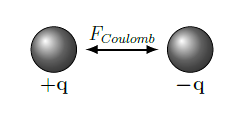
\includegraphics[scale=0.5]{image/chargecharge}	
\caption{Interaction électrostatique entre charges.}
\label{chargecharge}
\end{figure}



\begin{equation}
E_{Coulomb} = \frac{1}{4 \pi \epsilon_{0}} * \frac{q_{1} q_{2}}{r}
\end{equation}

\begin{flushleft}
\begin{tabular}{@{}lrp{10cm}}
avec & $q_{1}$ et $q_{2}$ : & charges respectives des particules 1 et 2, \\
& $r$ : & distance entre les particules. 
\end{tabular}
\end{flushleft}

L'induction est quant à elle due à la déformation de la densité électronique d'un atome ou d'une molécule par l'effet du champ électrique d'une molécule voisine. Ces deux contributions sont très bien définies en physique classique, contrairement à la dispersion et l'échange, qui sont liés à des effets quantiques.
En effet, ce sont les phénomènes de fluctuations quantiques de la distribution des charges qui sont à l'origine du terme de dispersion, et la contribution d'échange est dûe au principe d'exclusion de \textsc{Pauli} qui impose que deux électrons ne peuvent pas posséder le même état quantique au même moment. Dans le cas d'une paire d'atomes en interaction ayant leurs couches électroniques partiellement occupées, cette contribution est positive et engendre une liaison chimique liante forte. À l'inverse, lorsqu'il s'agit de systèmes électroniques à couche fermée, elle devient un terme de répulsion à courte distance responsable du phénomène d'exclusion stérique. Ce phénomène étant inclu dans la loi des \og gaz réels \fg{} de Van der Waals (équation~\ref{GR}) sous la forme du volume d'exclusion $nb$.  


D'une manière plus générale, c'est-à-dire en dépassant le cadre des gaz, les interactions de Van der Waals sont générées par les fluctuations de distributions de charge des atomes et molécules et conduisent aux équations suivantes, où l'énergie est exprimée en Joules :

\begin{align}
E_{Keesom} &= - \frac{1}{r^{6}} \left(\frac{\mu_{1}^{2}\mu_{2}^{2}}{3(4\pi \epsilon_{0} \epsilon)^{2} k_{B}T}\right) \\
E_{Debye} &= - \frac{1}{r^{6}} \left(\frac{\mu_{1}^{2}\alpha_{2}+\mu_{2}^{2}\alpha_{1}}{(4\pi \epsilon_{0} \epsilon)^{2}}\right) \\
E_{London} &= - \frac{1}{r^{6}} \left(\frac{3}{4}\frac{h\nu\alpha_{1}\alpha_{2}}{(4\pi \epsilon_{0})^{2}}\right)
\end{align}

\begin{flushleft}
\begin{tabular}{@{}lrp{10cm}}
avec & $\mu_{1}$ et $\mu_{2}$ : & moments dipolaires respectifs des particules 1 et 2, \\
& $\alpha_{1}$ et $\alpha_{2}$ : & polarisabilités respectives des particules 1 et 2, \\
& $\epsilon_{0}$ : & permittivité diélectrique du vide, \\
& $\epsilon$ : & permittivité diélectrique du milieu, \\
& $k_{B}$ : & constante de \textsc{Boltzmann}, égale à la constante des gaz parfaits $R$ divisée par le nombre d'\textsc{Avogadro} $\mathcal{N}\!a$, \\
& $T$ : & température, \\
& $r$ : & distance entre les particules. \\
\end{tabular}
\end{flushleft}

L'énergie de \textsc{Keesom} (effet d'orientation) représente l'énergie d'interaction entre deux dipôles électrostatiques, c'est-à-dire deux molécules ayant un moment dipolaire\footnote{Le moment dipôlaire d'une molécule résulte d'une répartition hétéroclite de charges électriques, telle que le barycentre des charges positives (noyaux) ne coïncide pas avec celui des charges négatives (électrons), les électrons étant en effet attirés par l'atome le plus électronégatif de la liaison.} $\mu{}$ non nul (figure~\ref{figKeesom}). Il s'agit concrètement de l'attraction mutuelle de deux dipôles permanents qui est d’autant plus forte que les moments dipolaires sont élevés (grande charge et petite taille de la molécule) et que la température est basse.

\begin{figure}[h]
\centering
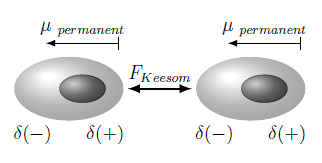
\includegraphics[scale=0.5]{image/Keesom}
\caption{Interaction entre dipôles électrostatiques.}
\label{figKeesom}
\end{figure}

Celle de \textsc{Debye} (effet d'induction) résulte de la déformation du nuage électronique d'une molécule, d'un atome ou d'un ion, par action du champ électrique engendré par le moment dipolaire d'une molécule voisine (figure \ref{figDebye}). Il en résulte ainsi un moment dipolaire induit. Elle est souvent nommé interaction dipôle {permanent-dipôle{ induit et fait intervenir le moment dipolaire $\mu$ et la polarisabilité\footnote{La polarisabilité est la capacité du nuage électronique à se déformer sous l'action d'un champ électrique. Le barycentre des charges négatives (électrons) étant légèrement décalé par rapport à celui des charges positives (noyaux) sous l'effet du champ, un moment électronique induit $\vec{m}_{e}$ apparaît, engendrant la notion de polarisabilité $\alpha$.} $\alpha$ des molécules concernées. Le nominateur $\mu_{1}^{2}\alpha_{2}+\mu_{2}^{2}\alpha_{1}$ décrit l'interaction lorsque les deux molécules sont polaires (cas A) mais s'écrit naturellement $\mu_{1}^{2}\alpha_{2}$ quand la seconde molécule est apolaire (cas B).

% mettre les deux cas dans la figure !
\begin{figure}[h]
\centering
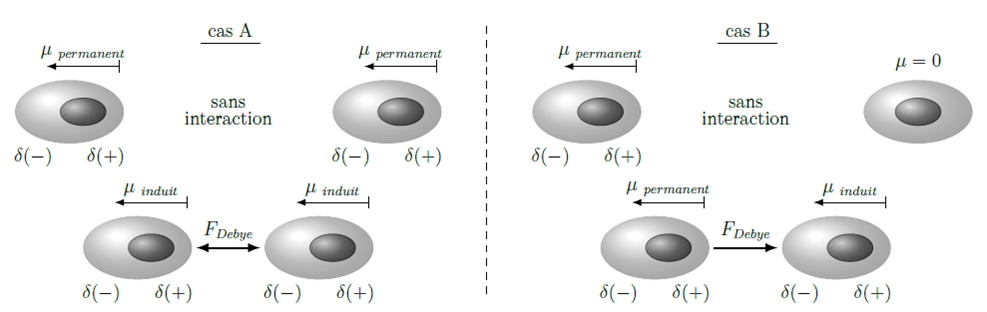
\includegraphics[scale=0.9]{image/Debye}
\caption{Interaction entre une molécule polaire et une seconde polarisable.}
\label{figDebye}
\end{figure}

Finalement, l'énergie de \textsc{London} (effet de dispersion), qui est la plus importante en terme de grandeur, représente l'interaction entre deux dipôles instantanés (figure \ref{figLondon}). Par définition, une molécule apolaire possède un moment dipolaire moyen nul mais la combinaison des mouvements des noyaux et des électrons fait qu'il existe malgré tout un moment dipolaire instantané. Cette interaction est d'autant plus forte que les deux molécules sont facilement polarisables, donc d'autant plus forte que leur taille est importante. Les forces de \textsc{London} étant présentes entre toutes les particules, quelle que soit leur nature, ce sont principalement elles qui permettent la cohésion de la matière dans l'univers.

Notons que les énergies de Van der Waals varient en fonction de l'inverse de la distance à l'ordre 6.

\begin{figure}[h]
\centering
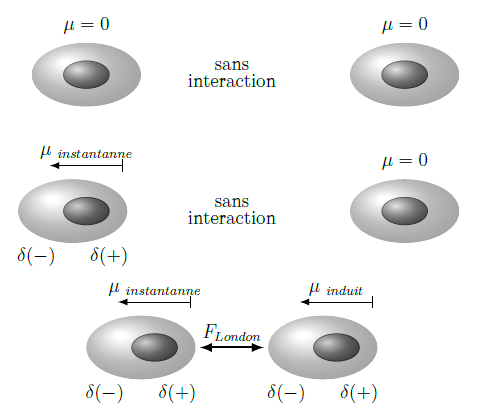
\includegraphics[scale=0.8]{image/London}
\caption{Interaction entre deux dipôles instantanés.}
\label{figLondon}
\end{figure}


Il existe toutefois d'autres types d'interactions électrostatiques que celles décrites par le modèle des forces de VdW. En effet, similaire dans l'esprit à l'énergie de \textsc{Keesom}, l'énergie d'interaction entre un ion et un dipôle permanent est donné par la formule suivante :

\begin{equation}
E_{ion-dipôle} = - \frac{1}{r^{2}} \frac{\mu_{1}q_{2}}{4\pi \epsilon_{0} \epsilon}
\end{equation} 

Il s'agit là encore de l'interaction positive entre une espèce chargée, anion ou cation, et une molécule possédant un moment dipolaire non-nul (\ref{figiondipole}). Ce phénomène est notamment à l'origine de la dissolution des espèces ioniques (ex~:~NaCl) dans un solvant polaire, de l'étape de solvatation qui suit, puis de la bonne dispersion des charges en solution.

\begin{figure}[h]
\centering
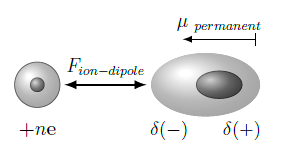
\includegraphics[scale=0.7]{image/Ion-dipole}
\caption{Interaction entre une espèce chargée et une molécule polaire.}
\label{figiondipole}
\end{figure}

De plus, notons aussi la spécificité de la liaison hydrogène qui est une liaison chimique non covalente, de type dipôle-dipôle. Lorsqu'un hétéroatome possédant au moins une paire libre est suffisamment électronégatif (ex : O, N, F), il vient se positionner aux abords d'un hydrogène acide porté par un autre atome fortement électronégatif afin d'en stabiliser la charge partielle $\delta (+)$ ainsi créée.

Bien que de la même famille que les forces de Van der Waals, \textit{i.e.} électrostatique, les liaisons hydrogènes s'en distinguent par une intensité environ dix fois supérieure. Elles restent toutefois une vingtaine de fois plus faibles qu'une liaison covalente. La distance moyenne entre les deux hétéroatomes est de l'ordre de 2,5 \AA .

Dans le cadre de cette thèse, ce sont principalement les interactions entre systèmes conjugués, \textit{i.e.} interactions $\pi-\pi$, qu'il sera nécessaire de traduire. Comme nous pouvons le voir dans le cas simple d'un dimère de benzène représenté en figure \ref{pistackbenz}, l'interaction positive se fait entre les liaisons $\sigma$ et les liaisons $\pi$ alors que les nuages électroniques des liaisons $\pi$ se repoussent naturellement, dû à leurs charges négatives.

Notons que nous retrouvons ce phénomène sous des aspects intramoléculaires, comme par exemple dans le cas de l'hyperconjugaison $\sigma-\pi$ qui vient stabiliser certaines conformations du toluène.

\begin{figure}[h]
\centering
\begin{tikzpicture}[scale=0.7, every node/.style={scale=0.7}]
\shade [shading=ball, ball color=gray, opacity=0.5] (0,0.8) ellipse (2.2cm and 0.6cm) ;
\draw (-2,1.2) --++ (1,0.5) --++ (2,0) --++ (1,-0.5) ;
\fill (-2,1.2) --++ (1,-0.6) --++ (2,0) --++ (1,0.6) --++ (-1,-0.5) --++ (-2,0) -- cycle ;
\draw [dashed] (0,1.2) ellipse (1.4cm and 0.35cm) ;
\shade [shading=ball, ball color=gray, opacity=0.5] (0,1.6) ellipse (2.2cm and 0.6cm) ;
\shade [shading=ball, ball color=gray, opacity=0.5] (0,-1.6) ellipse (2.2cm and 0.6cm) ;
\draw (-2,-1.2) --++ (1,0.5) --++ (2,0) --++ (1,-0.5) ;
\fill (-2,-1.2) --++ (1,-0.6) --++ (2,0) --++ (1,0.6) --++ (-1,-0.5) --++ (-2,0) -- cycle ;
\draw [dashed] (0,-1.2) ellipse (1.4cm and 0.35cm) ;
\shade [shading=ball, ball color=gray, opacity=0.5] (0,-0.8) ellipse (2.2cm and 0.6cm) ;
\draw [latex-latex, thick] (-2.2,-1.2) ..controls +(-1.7,0) and +(-1.5,0).. (-2.4,0.8) node [above, midway, rotate=90, yshift=3mm] {interaction attractive $\sigma - \pi$} ;
\draw [latex-latex, thick] (-2.2,1.2) ..controls +(-1.7,0) and +(-1.5,0).. (-2.4,-0.8) ;
\draw [latex-latex, thick] (2.4,-0.8) ..controls +(1.5,0) and +(1.5,0).. (2.4,0.8) node [below, midway, rotate=90, yshift=-2mm] {interaction répulsive $\pi - \pi$} ;
\end{tikzpicture}
\caption{$\pi$-stacking dans le cas d'un dimère de benzène}
\label{pistackbenz}
\end{figure}

Même si la théorie de la fonctionnelle de la densité connaît un large succès tant elle arrive désormais bien à traduire les phénomènes de liaisons chimiques, les structures géométriques et même la cohésion des solides moléculaires et cristallins, il reste toujours l'obstacle des systèmes chimiques où les forces de Van der Waals sont prédominantes. En effet, les effets de corrélation électronique des forces de dispersion étant purement non-locaux, l'approximation locale ou non-locale qui fait le fondement de la DFT restera problèmatique. Se pose alors la question de savoir comment modéliser ces types d'interaction de façon idiomatique. Nous allons voir que l'élaboration d'une fonctionnelle hybride à longue portée est capable de répondre à cette problèmatique.

\section[LC-DFT-D hybride : $\omega$BXD]{Construction d'une LC-DFT-D hybride : cas de la $\omega$BXD}

Les DFT hybrides avec correction à longue portée basées sur la théorie \textsc{Kohn-Sham} ont naturellement rencontré un grand engouement puisque la précision apportée n'accroît pas le coût calculatoire par rapport aux DFT hybrides.

\subsection{B88}

Comme nous l'avons vu dans le cadre des approximations de la fonctionnelle de la densité, notées DFAs\footnote{\og Density Functional Approximations \fg{} }, la décroissance en exponentielle du potentiel d'échange-corrélation, au lieu d'être en $1/r$, engendre une mauvaise représentation des interactions à longue distance. Cette erreur, nommée erreur d'auto-interaction (SIE, pour \og self-interaction error \fg{}), est liée au fait que ces approximations, basées sur la densité de spin locale (LSDA, pour \og local spin density approximation \fg{}), décrivent mal l'état fondamental qui devrait être, dans le cadre de la DFT pure, strictement sans auto-interaction.     
C'est pourquoi, afin d'introduire un effet non-local de l'échange-corrélation dans le modèle KS-DFT (partie~\ref{Kohn-Sham}), \textsc{Becke} proposa en 1988 d'incorporer dans sa fonctionnelle d'échange B88~\cite{becke1988density} une petite part d'echange exact \textsc{Hartree-Fock}. 

Dans le cadre général des DFAs, l'énergie d'échange-corrélation s'écrit donc :

\begin{equation}
E_{xc} = c_{x}E_{x}^{HF} + E_{xc}^{DFA}
\label{xcB88}
\end{equation}

\noindent où $c_{x}$ prend généralement des valeurs comprises entre 0,2 et 0,25~\cite{becke1993density} pour les données thermodynamiques et entre 0,4 et 0,6~\cite{boese2004development} pour les études cinétiques.

Basée sur ce modèle, la désormais bien connue DFT hybride B3LYP \cite{becke1993density} (équation~\ref{B3LYP}) donne des résultats comparables à ceux obtenus à partir de la théorie perturbative \textsc{M\o ller-Plesset} à l'ordre 2 \cite{moller1934note}, noté MP2, souvent utilisée comme référence, dans le cadre de systèmes fortement liés. Depuis, de nombreuses recherches ont porté sur l'amélioration constante de ce potentiel d'échange-corrélation $E_{xc}[\rho]$.

\subsection{B97}

Une avancée significative a de nouveau été faite par \textsc{Becke} en 1997 dans le domaine des KS-DFT. Par une méthode similaire à la combinaison linéaire d'orbitales atomiques, notée LCAO\footnote{\og Linear Combination of Atomic Orbitals \fg{}.}, il a proposé un modèle mathématique basé sur l'approximation de densité de spin local (LSDA), sa première dérivée et une petite fraction d'échange HF pour décrire le potentiel d'échange-corrélation $E_{xc}[\rho]$. Une optimisation systématique des coefficients linéaires à partir d'un jeu classique de données expérimentales a conduit à l'apparition de la méthode B97~\cite{becke1997density}. La base de données contient notamment des valeurs relatives à l'interaction entre systèmes conjugués.

Cette méthodologie a été reprise par F. A. \textsc{Hamprecht} et al, P. J. \textsc{Wilson} et al et T. W. \textsc{Keal} et al pour respectivement conduire à la B97-1 \cite{hamprecht1998development} (1998), la B97-2 \cite{wilson2001hybrid} (2001) et la B97-3 \cite{keal2005semiempirical} (2005). Il s'agissait alors de réoptimisations des coefficients linéaires par rapport à d'autres bases de données expérimentales plus complètes.

Mais cette reparamétrisation empirique du terme d'échange-corrélation ne résout pas le problème de sa non-décroissance en $1/r$. La prise en compte totale du terme d'échange HF $E_{x}^{HF}$ ($c_{x}$=1 dans l'équation~\ref{xcB88}) pourait résoudre ce problème mais cela serait incompatible avec le terme de corrélation DFA $E_{c}^{DFA}$. En effet, il existerait alors une mauvaise compensation des erreurs respectives.

\subsection{$\omega$B97}

L'idée de séparer le traitement des interactions courtes (SR, pour \og short range \fg{}) et longues portées (LR, pour \og long range \fg{}) s'est alors présentée comme le choix le plus évident, aussi bien au niveau de la compréhension des phénomènes que mathématiquement parlant. Nous pouvons ainsi traiter séparément à l'aide d'une fonction erreur $(erf)$ les interactions à courtes distances par une fonctionnelle de la densité et celles longue distance par une fonction d'onde. Ce principe conduit naturellement à l'élaboration d'une fonctionnelle hybride à séparation de portée. L'introduction de la fonction erreur, avec un paramètre libre, permet de contrôler le rayon d'action des interactions de courte-portée.

La première proposition faite par \textsc{Iikura} et al \cite{iikura2001long} a été de traiter la partie d'échange LR par la théorie HF alors que la partie SR est approximée par une DFA; le terme de corrélation est quant à lui le même que celui de \textsc{Coulomb}, quelle que soit la distance :

\begin{equation}
E_{xc}^{LC-DFA} = E_{x}^{LR-HF} + E_{x}^{SR-DFA} + E_{c}^{DFA}
\end{equation}

Ce schéma de séparation de portée a l'avantage de conduire à des temps de calcul très proches des DFT hybrides, mais il reste à développer une fonctionnelle d'échange SR précise et une fonctionnelle de corrélation qui soit entièrement compatible entre elles.

Le type d'opérateur de coupure le plus utilisé dans le cadre des LC-DFT hybrides est la fonction d'erreur standard $(erf)$ :

\begin{equation}
\frac{1}{r} = \frac{erf(\omega r_{12})}{r_{12}} + \frac{erfc(\omega r_{12})}{r_{12}}
\label{erf}
\end{equation}

\begin{flushleft}
\begin{tabular}{@{}lrp{10cm}}
avec & $\frac{erf(\omega r_{12})}{r_{12}}$ : & interaction de courte portée, \\
& $\frac{erfc(\omega r_{12})}{r_{12}}$ : & interaction complémentaire, \\
& $r_{12}$ : & distance entre les particules 1 et 2, \\
& $\omega$ : & paramètre contrôlant la séparation.
\end{tabular}
\end{flushleft}

Notons que l'introduction du paramètre $\omega$, qui s'exprime comme l'inverse d'une distance, permet de donner un sens physique à cette valeur, en cela qu'il est étroitement lié à une longueur caractéristique de la séparation.
Naturellement, il existe différents types de fonctions erreur $(erf)$ afin de faciliter son intégration mathématique dans les codes de calculs. Dans le cas de la $\omega$B97 \cite{chai2008long} et, par conséquent, des fonctionnelles $\omega$B97X et $\omega$B97X-D, c'est la fonction $erf/erfc$ qui a été choisie par Jeng-Da \textsc{Chai} et Martin \textsc{Head-Gordon} dans leurs travaux. \\

Le choix des auteurs s'est porté sur un terme d'échange exact HF longue portée $E_{x}^{LR-HF}$, calculé à partir des spin-orbitales occupées $\phi_{i \sigma}(r)$, et une forme analytique du terme d'échange $E_{x}^{SR-DFA}$ obtenue par l'intégration du carré de la matrice densité LSDA :

\begin{align}
E_{x}^{LR-HF} &= -\frac{1}{2} \sum_{\sigma} \sum_{ij}^{occ.} \iint \phi_{i \sigma}^{*}(r_{1}) \phi_{j \sigma}^{*}(r_{1}) \frac{erf(\omega r_{12})}{r_{12}} \phi_{i \sigma}(r_{2}) \phi_{j \sigma}(r_{2}).dr_{1}.dr_{2}, \\
E_{x}^{SR-LSDA} &= \sum_{\sigma} \int \underbrace{-\frac{3}{2}\left(\frac{3}{4\pi}\right)^{1/3}\rho_{\sigma}^{4/3} (r) F(a_{\sigma})}_{e_{x \sigma}^{SR-LSDA} (\rho_{\sigma}) .dr}.
\end{align}

\noindent où :
\begin{align}
k_{F \sigma}&=(6\pi^{2}\rho_{sigma}(r))^{1/3},\nonumber\\
F(a_{\sigma})&=1-\frac{8}{3}a_{\sigma}\left[\sqrt{\pi}\: erf\left(\frac{1}{2a_{\sigma}}\right)-3a_{\sigma}+4a_{\sigma}^{3}+(2a_{\sigma}-4a_{\sigma}^{3}) \: exp\left(-\frac{1}{4a_{\sigma}^{2}}\right)\right],\nonumber\\
a_{\sigma}&=\frac{\omega}{2k_{F\sigma}}.\nonumber
\end{align}

\begin{flushleft}
\begin{tabular}{@{}lrp{10cm}}
avec & $k_{F\sigma}$ : & vecteur d'onde local de Fermi,\\
& $F(a_{\sigma})$ : & fonction d'atténuation,\\
& $a_{\sigma}$ : & paramètre de contrôle (sans unité) de la fonction d'atténuation $F(a_{\sigma})$.
\end{tabular}
\end{flushleft}

En retenant une fonctionnelle de corrélation basée elle aussi sur la LSDA $E_{c}^{LSDA}$, la plus simple des DFT hybrides à correction de longue portée (RSHX-LDA) s'écrit~:

\begin{equation}
E_{xc}^{RSHXLDA} = E_{x}^{LR-HF} + E_{x}^{SR-LSDA} + E_{c}^{LSDA}
\end{equation}

La fonctionnelle $\omega$B97\cite{chai2008long} s'écrit alors :

\begin{equation}
E_{xc}^{\omega B97} = E_{x}^{LR-HF} + E_{x}^{SR-B97} + E_{c}^{B97}
\end{equation}

Il est à noter que celle-ci ne possède pas d'échange \textsc{Hartree-Fock} à courte portée (SR), comme la plupart des fonctionnelles hybrides à correction de portée.

Malgré plusieurs études visant à optimiser la valeur du paramètre $\omega$, la précision calculatoire reste insuffisante en terme de thermochimie. En effet, nous l'avons déjà vu, une valeur trop grande pour $\omega$ tendrait vers une incompatibilité entre le terme d'échange non-local $E_{x}^{LR-HF}$ et le terme local de corrélation $E_{c}^{LSDA}$. De plus, nous pouvons aisément comprendre, d'après l'équation~\ref{erf}, que plus $\omega$ est petit, plus la contribution du terme d'échange SR $E_{x}^{SR-LSDA}$ sera importante. L'utilisation d'une trop faible valeur  reviendrait alors à traiter le problème dans un cadre très proche de la LDA classique qui, comme nous l'avons vu dans la partie~\ref{lda}, est incapable de traduire correctement le terme d'échange à courte portée.

\subsection{$\omega$B97X}

Afin d'y remédier, une partie d'échange SR HF $E_{x}^{SR-HF}$, est ajoutée à $E_{x}^{SR-LSDA}$ dans une proportion d'environ 16\%,  de la même manière que \textsc{Becke} dans la fonctionnelle B88. Ceci à l'avantage de ne pas perturber la partie LR qui est dorénavant correcte. Ainsi, la nouvelle fonctionnelle comporte désormais un paramètre $c_{x}$ contrôlant la proportion d'échange exact HF à courte distance, comme nous pouvons le voir dans son expression :

\begin{equation}
E_{xc}^{LC-DFA} = E_{x}^{LR-HF} + c_{x}E_{x}^{SR-HF} + E_{x}^{SR-DFA} + E_{c}^{DFA}
\end{equation}

\noindent où :

\begin{equation}
E_{x}^{SR-HF} = -\frac{1}{2} \sum_{\sigma} \sum_{ij}^{occ.} \iint \phi_{i \sigma}^{*}(r_{1}) \phi_{j \sigma}^{*}(r_{1}) \frac{erfc(\omega r_{12})}{r_{12}} \phi_{i \sigma}(r_{2}) \phi_{j \sigma}(r_{2}).dr_{1}.dr_{2}, \\
\end{equation}

C'est ainsi que la fonctionnelle $\omega$B7X\cite{chai2008long} se décompose de la façon suivante~:

\begin{equation}
E_{xc}^{\omega B97X} = E_{x}^{LR-HF} + c_{x}E_{x}^{SR-HF} + E_{x}^{SR-B97} + E_{c}^{B97}
\end{equation}

La valeur de $\omega$, comme les valeurs des coefficients de développements linéaires et de développements à l'ordre $m$ des fonctionnelles $\omega$B97 et $\omega$B97X ont été déterminées par la méthode des moindres carrés appliquée à une base de données composées de 412 valeurs précises, expérimentales et théoriques.

Malgré toutes ces optimisations conduisant à une bien meilleure représentation des systèmes en interaction, ces fonctionnelles connaissent encore des lacunes quant à la traduction des interactions de dispersion entre atomes, ie les forces de \textsc{London}. Comme nous allons le voir dans le cas de la fonctionnelle $\omega$B97X-D, ceci peut être corrigé par une prise en compte empirique des effets de dispersion.

\subsection{$\omega$B97X-D}

Cette dernière correction pourrait naturellement passer par le calcul idiomatique de l'énergie de dispersion entre chaque atome, mais cela occasionnerait alors un coût calculatoire prohibitif. C'est pourquoi Jeng-Da \textsc{Chai} et Martin \textsc{Head-Gordon} ont fait le choix d'appliquer cette correction de façon empirique par l'ajout d'un terme $E_{disp}$ à la fonctionnelle KS-DFT, ici la $\omega$B97X. L'expression de l'énergie de la fonctionnelle $\omega$B97X-D \cite{chai2008long} ainsi créée devient alors :

\begin{equation}
E_{DFT-D}=E_{\omega B97X}+E_{disp}
\end{equation}

L'énergie de dispersion $E_{disp}$ est définie par rapport à une fonction d'amortissement $f_{damp}$ :

\begin{equation}
E_{disp}=-\sum_{i-1}^{N_{at}-1} \sum_{j-i+1}^{N_{at}} \frac{C_{6}^{ij}}{R_{ij}^{6}}f_{damp} (R_{ij})
\end{equation}

\noindent où :
\begin{equation}
f_{damp} (R_{ij})=\frac{1}{1+a(\frac{R_{ij}}{R_{r}})^{-12}}
\end{equation}

Une nouvelle fois, la partie empirique a été paramétrée par rapport à la même base de données que pour les fonctionnelles $\omega$B97 et $\omega$BX97.


\newpage

\section*{Conclusion}
\markright{CONCLUSION}{}

En résumé, l'apport de la fonction erreur $(erf)$ permet de mieux gérer les contributions d'échange-corrélation selon la distance d'interaction. Les DFT hybrides $\omega$B97 et $\omega$B97X prennent ainsi en compte la totalité de l'échange exact à longue distance et utilisent la méthode des gradients généralisés à faible distance, alors que la corrélation électronique reste basée sur celle initialement développée par \textsc{Becke} dans la fonctionnelle B97. Ceci a pour effet de supprimer le problème d'auto-interaction de la fonctionnelle d'échange à longue distance.

Les travaux de Jeng-Da \textsc{Chai} et Martin \textsc{Head-Gordon} ont finalement conduit à la fonctionnelle $\omega$B9X-D, de type LC-DFT-D hybride, où la totalité de l'échange exact HF est pris en compte à longue distance, en même temps qu'une petite partie -- environ 22 \% -- de l'échange exact HF est introduite à courte distance pour compléter une fonctionnelle d'échange B97 modifiée ; une correction empirique de la dispersion est finalement appliquée.

Comme toutes les fonctionnelles LC-DFT, le problème de l'auto-interaction est corrigé à longue distance mais reste quelque peu présent à courte distance. Les effets de corrélation à longue distance sont quant à eux purement et simplement traités par la correction empirique de dispersion.

Cette fonctionnelle est, d'après les tests des auteurs, définitivement plus adaptée à l'étude de systèmes chimiques où les interactions non-covalentes sont importantes.







\newgeometry{textwidth=16cm}
\chapter{Partie vibrationnelle}
\minitoc
\restoregeometry

\newpage


% % % % % % % % % % % % % % % % % % % % % % % % % % % % % % % % % % % % % % % % % % % % % % % % % % % % % % % % 
% % % % % % % % % % % % % % % % % % % % % % % % % % % % % % % % % % % % % % % % % % % % % % % % % % % % % % % % 
% % % % % % % % % % % % % % % % % % % % % % % % % % % % % % % % % % % % % % % % % % % % % % % % % % % % % % % % 

\section*{Introduction}
\markright{INTRODUCTION}{}
\spacing{1.5}
La littérature consacrée aux applications des spectrométries vibrationnelles dans le domaine de la caractérisation des constituants présent dans les pétroles est relativement peu abondante même si la spectrométrie infrarouge est devenue une technique d'analyse de \og routine \fg{} dans de très nombreux laboratoires, académiques comme industriels. La raison de cette faible abondance réside essentiellement dans le fait de la complexité des mélanges qui constituent un pétrole, un asphaltène … Pourtant les champs de cette technique d'applications se sont considérablement développés depuis l'apparition sur le marché de spectrophotomètres à transformée de \textsc{Fourier}.
Après avoir vu sa position privilégiée menacée par d'autres méthodes, telles que la spectroscopie RMN\footnote{\og Nuclear Magnetic Resonance Spectroscopy \fg{}.} ou la spectrométrie de masse, la spectrométrie infrarouge à transformée de \textsc{Fourier} (IRTF) a connu de nouvelles avancées technologiques, telle que la spectrométrie photoacoustique que nous avons employés dans ce travail, qui lui confèrent à l'heure actuelle une précision d'analyse permettant d'atteindre des informations détaillées sur :

\begin{itemize}
	\item la structure chimique de molécules, de macromolécules: identification de l'unité de base, des ramifications ; analyses des extrémités de chaînes ; identification des défauts, d'éventuelles impuretés\dots{}
	\item les interactions intra et inter-moléculaires, la conformation des chaînes, l'orientation des molécules et des macromolécules, les auto-associations éventuelles, \textit{etc}\dots{}
\end{itemize}

Cette partie a pour but essentiel de définir le vocabulaire et les notions fondamentales que nous emploierons par la suite, le développement détaillé du traitement classique de la vibration se trouvant dans de nombreux ouvrages  et repris dans de nombreuses thèses. Parallèlement à ces développements expérimentaux, la modélisation en spectroscopie vibrationnelle a connu ces dernières décennies de très grandes mutations. Ce chapitre vise aussi à rappeler les fondements essentiels de la résolution de l'équation vibrationnelle de Schr\"{o}dinger, qui sous-tendent les principales méthodes -- que nous développerons -- actuellement disponibles pour tenter de répondre aux problématiques posées par les expérimentateurs. 


En particulier, le domaine de la pétrochimie qui nous intéresse dans ce travail, et précisément la thématique visant à l'élucidation de la composition de ces mélanges complexes et composés de milliers de molécules différentes non encore identifiées, est un domaine au champ d'investigation large et pour lequel les attentes sont grandes en termes de caractérisation comme en terme de compréhension des processus d’interaction et d’agrégation de ces molécules. Dans ce domaine encore, la spectrométrie IRTF est certainement un des outil le plus efficace pour élucider les mécanismes impliqués, mais les données résultantes sont complexes et de fait difficilement interprétables et justifiables sans un support théorique adapté.

L'Équipe de Chimie Physique (ECP) de l'IPREM est depuis très longtemps spécialisée dans les développements méthodologiques et logiciels dans la double hypothèse des anharmonicités électriques et mécaniques. Pour ces compétences, les expérimentateurs  font généralement appel à la modélisation, dans le but d'interpréter leurs données spectrales.
Le problème qui nous a été posé dans ce travail a cependant constitué un challenge qui nous a contraint à adapter nos méthodes de calculs pour proposer, \textit{in fine}, une méthode de type variation-perturbation adaptée et simplifiée permettant une interprétation des données dans des gammes spectrales non usuelles (très bas nombres d’ondes) et sur un ensemble de molécules suffisamment large et représentatif de quelques familles moléculaires suspectées comme étant présentent dans les asphaltènes. 


\newpage

% % % % % % % % % % % % % % % % % % % % % % % % % % % % % % % % % % % % % % % % % % % % % % % % % % % % % % % % 
% % % % % % % % % % % % % % % % % % % % % % % % % % % % % % % % % % % % % % % % % % % % % % % % % % % % % % % % 
\section{Généralités}

L'identification des principaux composés -- ou, pour le moins, des familles de composés -- chimiques fait l'objet, depuis de nombreuses années, de recherches intensives.

En soit, la thématique liée à l'identification et à la caractérisation des molécules au sein d'un milieu chimique donné n'a rien de novatrice. En effet, depuis de nombreuses décennies, les chimistes de tous domaines recherchent ce \og graal \fg{} avec plus ou moins de succès. Parmi les techniques expérimentales les plus utilisées pour répondre au problème, la spectroscopie vibrationnelle est certainement celle qui a permis le plus grand nombre de progrès dans des domaines aussi variés que la biochimie, l'agroalimentaire, la chimie interstellaire ou encore la chimie des matériaux. Le point commun à l'ensemble de ces études est qu'elles sont toutes basées sur une connaissance \textit{a minima} des molécules constituant le milieu étudié. La complexité des problèmes de suivi et de devenir d’un ensemble de molécules mal défini et ayant évolué dans des conditions extrêmes sur une échelle de temps démesurée (en terme de réactivité chimique) rend toutefois l'utilisation de cette technique plus délicate et plus hasardeuse, si bien qu'il est indispensable de faire appel à des techniques complémentaires ou de recourir au soutien de la modélisation prédictive. Il est en effet indéniable que les progrès conjoints des techniques de modélisation et des moyens informatiques font aujourd'hui de cet outil un support indispensable et performant à l'identification de systèmes moléculaires de plus en plus variés.\\

Le développement de ces modélisations en spectroscopie vibrationnelle fait état depuis une vingtaine d'années de progrès fulgurants. Les techniques mathématiques développées par les générations précédentes sont désormais largement éprouvées et mises en application au service des expérimentateurs.
Il ne se passe plus une seule année sans que les limites calculatoires et les précisions atteintes par ces simulations ne soient repoussées, grâce au développement de méthodes adaptées et développées dans le cadre d'hypothèses mathématiques précises et contrôlées. \\

Le travail présenté dans ce chapitre s'inscrit donc dans le cadre de ces développements mathématiques au service de l'identification de systèmes chimiques complexes. Les calculs que nous développons sont réalisés dans le cadre de la Résolution de l'Equation vibrationnelle de Sch\"{o}dinger (RES), dans la double hypothèse des approximations anharmoniques électriques et mécaniques permettant d'accéder à la détermination des intensités et des fréquences de tous les modes de vibrations intrinsèques à un système chimique donné, dans un environnement donné. Il est encore communément admis qu'un calcul mené dans une hypothèse plus simple, dite harmonique, suffit aux identifications. En réalité, les raisons fondamentales qui poussent les chercheurs à préférer l'approximation harmonique sont aussi bien liées au problème de coût calculatoire autant qu'au manque d'implémentation d'approches de type anharmoniques dans les grands codes de calculs commerciaux. Dans la stratégie que nous développons, nos calculs se distinguent des études menées dans le domaine en cela qu'ils se placent précisément dans l'hypothèse anharmonique. Néanmoins, il est important de savoir qu'un calcul réalisé dans l'hypothèse harmonique engendre une erreur que le modélisateur à pour habitude de \og contrôler \fg{} par un facteur correctif adapté qu'il applique à ses résultats selon les conditions de calculs utilisées lors de la RES. Malheureusement, cette technique de calcul, utilisée depuis une cinquantaine d'années, et qui a fait de la modélisation en spectroscopie vibrationnelle une méthode quelque peu empirique dans l'esprit des expérimentateurs, est toujours assujettie à un doute quant à l'identification précise des vibrateurs, car il n'est fondamentalement pas concevable que l'erreur commise sur chaque mode soit la même pour tous et que la correction proposée soit universellement applicable à tous les système étudiés quels que soient les milieux dans lesquels ils se trouvent. De plus, les calculs développés dans cette hypothèse ne permettent pas d'identifier d'autres vibrateurs que les modes fondamentaux puisqu'aucun couplage entre modes n'est pris en compte.

En résumé, toute modélisation en spectroscopie vibrationnelle, qu’elle soit développée dans l’hypothèse harmonique ou anharmonique, est directement dépendante de la qualité de la fonction d’onde moléculaire électronique, donc de la prise en compte de la corrélation électronique. S’il est aujourd’hui commun de réaliser la REVS pour des systèmes de petite taille (3, 4 atomes), ce critère devient toutefois pratiquement rédhibitoire lorsqu'il s'agit de résoudre ces mêmes problèmes dans l’hypothèse anharmonique sur des systèmes de taille plus importante.

Ce chapitre constituera avant tout une occasion pour moi de recenser les difficultés inhérentes au développement méthodologique vibrationnel et de montrer les pistes avancées pour l'étude des systèmes moléculaires dont la taille excède la vingtaine d'atomes, taille minimale nécessaire à la caractérisation des motifs/familles de base présentes dans les asphaltènes. Ces activités s’inscrivent dans le prolongement et le complément des actions antérieures menées au sein de l'ECP, notamment pour le développement de méthodes de variation-perturbation et de calcul des intensités IR de petits systèmes moléculaires \ref{krusic1991electron}. 



% % % % % % % % % % % % % % % % % % % % % % % % % % % % % % % % % % % % % % % % % % % % % % % % % % % % % % % % 
% % % % % % % % % % % % % % % % % % % % % % % % % % % % % % % % % % % % % % % % % % % % % % % % % % % % % % % % 
\section[Séparation des mouvements]{Séparation des mouvements rotationnels et vibrationnels}

Cette partie a pour but essentiel de définir le vocabulaire et les notions fondamentales que nous emploierons par la suite, le développement détaillé du traitement classique de la vibration se trouvant dans de nombreux ouvrages~\cite{barchewitz1971spectroscopie,wilson1955molecular,wilson1955molecular} et repris dans de nombreuses thèses~\cite{pouchan1978approche,zaki1996etude}.

Dans une approximation d'ordre 0 supplémentaire à celle de \textsc{Born}- \textsc{Oppenheimer}, les mouvements nucléaires peuvent être séparés en deux classes : les mouvements de rotation et les mouvements de vibration.
Pour ce faire, il est nécessaire d'expliciter l'expression de l'énergie cinétique des noyaux au sens classique et de repérer la molécule dans un référentiel respectant les conditions d'\textsc{Eckart}~\cite{eckart1935some}
Considérons dans cet espace un repère mobile $oxyz$, lié à la molécule, et un repère fixe $OXYZ$, définissant les mouvements de translation et de rotation du repère mobile. Le mouvement du trièdre mobile par rapport au trièdre fixe est défini par la distance $R$ et la vitesse angulaire instantanée $\alpha$.
Le mouvement de la molécule est défini par le trièdre mobile représentant à chaque instant la position $\stackrel{\rightarrow}{r_{\alpha}}$ des noyaux $\alpha$ par rapport à leur position d'équilibre $\stackrel{\rightarrow}{a_{\alpha}}$. Soit : 

\begin{equation}
\stackrel{\rightarrow}{\rho_{\alpha}} = \stackrel{\rightarrow}{r_{\alpha}} - \stackrel{\rightarrow}{a_{\alpha}}
\end{equation}

La vitesse $\stackrel{\rightarrow}{v_{\alpha}}$ du $\alpha^{ieme}$ noyau est donc : $\stackrel{\rightarrow}{v_{\alpha}} =\stackrel{\rightarrow}{\dot{r_{\alpha}}} =  \stackrel{\rightarrow}{\dot{\rho_{\alpha}}}$ puisque, par définition, $\stackrel{\rightarrow}{a_{\alpha}}$ est constant dans le temps.
	
Ainsi, dans le repère fixe, la vitesse de ce noyau s'écrit :
	
\begin{equation}
	\stackrel{\rightarrow}{V_{\alpha}} = \stackrel{\rightarrow}{\dot{R}} + \left(\stackrel{\rightarrow}{\omega} \wedge \stackrel{\rightarrow}{r_{\alpha}}\right) + \stackrel{\rightarrow}{v_{\alpha}}
\end{equation}

On peut facilement déduire de cette expression l'énergie cinétique totale des noyaux :

\begin{align}\label{2T-Eckart}
	2T = \dot{R}^2 \sum_{\alpha}m_{\alpha}\left(\stackrel{\rightarrow}{\omega} \wedge \stackrel{\rightarrow}{r_{\alpha}}\right)^2 &+ \sum_{\alpha}m_{\alpha}v^2_{\alpha} \\ \notag
	 &+ 2\stackrel{\rightarrow}{\dot{R}}\sum_{\alpha}m_{\alpha}\stackrel{\rightarrow}{v_{\alpha}} \\ \notag 
	 &+ 2\left(\stackrel{\rightarrow}{\dot{R}} \wedge  \stackrel{\rightarrow}{\omega}\right)\sum_{\alpha}m_{\alpha}\stackrel{\rightarrow}{r_{\alpha}} \\ \notag
	 &+ 2\stackrel{\rightarrow}{\omega}\sum_{\alpha}m_{\alpha}\left(\stackrel{\rightarrow}{r_{\alpha}} \wedge \stackrel{\rightarrow}{v_{\alpha}}\right)
\end{align}

Si nous supposons que les noyaux ne possèdent aucun mouvement de translation dans le système mobile et que l'origine de ce dernier correspond au centre de gravité de la molécule, alors :

\begin{equation}
	\sum_{\alpha}m_{\alpha}\stackrel{\rightarrow}{v_{\alpha}} = 0
\end{equation}
\noindent et
\begin{equation}
	\sum_{\alpha}m_{\alpha}\stackrel{\rightarrow}{r_{\alpha}} = 0
\end{equation}

Si, de plus, nous considérons que dans le trièdre mobile la molécule ne possède aucun mouvement de rotation, nous pouvons écrire :

\begin{equation}
	\sum_{\alpha}m_{\alpha}\left(\stackrel{\rightarrow}{a_{\alpha}} \wedge \stackrel{\rightarrow}{v_{\alpha}}\right) = 0
\end{equation}
\noindent et donc
\begin{equation}
	\sum_{\alpha}m_{\alpha}\left(\stackrel{\rightarrow}{r_{\alpha}} \wedge \stackrel{\rightarrow}{v_{\alpha}}\right) = \sum_{\alpha}m_{\alpha}\left(\stackrel{\rightarrow}{\rho_{\alpha}} \wedge \stackrel{\rightarrow}{v_{\alpha}}\right)
\end{equation}

Les deux conditions ci-dessus portent le nom de conditions d'\textsc{Eckart} et simplifient l'expression~\ref{2T-Eckart} :
	
\begin{equation}
	2T = \dot{R}^2\sum_{\alpha}m_{\alpha} + \sum_{\alpha}m_{\alpha}\left(\stackrel{\rightarrow}{\omega} \wedge \stackrel{\rightarrow}{r_{\alpha}}\right)^2 + \sum_{\alpha}m_{\alpha}v^2_{\alpha} + 2\stackrel{\rightarrow}{\omega}\sum_{\alpha}m_{\alpha}\left(\stackrel{\rightarrow}{r_{\alpha}} \wedge \stackrel{\rightarrow}{v_{\alpha}}\right)
\end{equation}

Le premier terme correspond à l'énergie cinétique de translation de la molécule. Il ne contribue pas à la quantification de l'énergie. Le second terme correspond  à l'énergie cinétique de rotation. Le troisième terme correspond à l'énergie de vibration moléculaire. Le dernier terme est appelé terme de \textsc{Coriolis}. Il est relatif à l'interaction entre la rotation et la vibration, et peut être négligé si nous considérons que les mouvements vibrationnels sont de faible amplitude : $\stackrel{\rightarrow}{r_{\alpha}} \approx \stackrel{\rightarrow}{a_{\alpha}}$. Cette approximation  appelée condition de \textsc{Casimir}~\cite{casimir1931rotation} est généralement vérifiée pour les vibrations d'élongation, par opposition aux modes très mous de torsion, qui restent souvent mal traduits dans ce cadre.
En conséquence, l'énergie cinétique des noyaux peut s'écrire, en première approximation, comme la somme d'un terme rotationnel et d'un terme vibrationnel :

\begin{equation}
	2T_n = 2T_R + 2 T_V \text{ en supposant }2T_{VR} = 0
\end{equation}

D'un point de vue quantique, les considérations ci-dessus conduisent à séparer les mouvements rotationnels et vibrationnels de l'équation nucléaire en deux équations distinctes :

\begin{align}
	\psi^n_{R_{\alpha}} &= \psi^R_{R_{\alpha}} \bullet \psi^V_{R_{\alpha}} \\
	E_n &= E_V + E_R
\end{align}
\begin{flushleft}
\begin{tabular}{@{}lrp{10cm}}
avec & $\psi^R_{R_{\alpha}}$ : & fonction d'état rotationnelle, \\
& $\psi^V_{R_{\alpha}}$ : & fonction d'état vibrationnelle,\\
& $E_R$ : & énergie correspondant à la fonction d'état rotationnelle,\\
& $E_V$ : & énergie correspondant à la fonction d'état vibrationnelle.
\end{tabular}
\end{flushleft}

On obtient ainsi l'équation de Schr\"{o}dinger décrivant les mouvements vibrationnels :

\begin{equation}
	\left(\hat{T}_V + \hat{V}_V\right) \psi^V_{R_{\alpha}} = E_V \psi^V_{R_{\alpha}}
\end{equation}

\noindent et l'équation de Schr\"{o}dinger décrivant les mouvements rotationnels dans l'hypothèse où les liaisons interatomiques ne s'allongent pas pendant la rotation (hypothèse du rotateur rigide):

\begin{equation}
	T_R \psi^R_{R_{\alpha}} = E_R \psi^R_{R_{\alpha}}
\end{equation}


% % % % % % % % % % % % % % % % % % % % % % % % % % % % % % % % % % % % % % % % % % % % % % % % % % % % % % % % 
% % % % % % % % % % % % % % % % % % % % % % % % % % % % % % % % % % % % % % % % % % % % % % % % % % % % % % % % 
\section{Energie cinétique de vibration }

L'énergie cinétique de vibration d'une molécule composée de $n$ atomes dans le repère d'\textsc{Eckart} s'écrit :

\begin{equation}
	2T_V = \sum^n_{\alpha}m_{\alpha}\left( \dot{x}^2_{\alpha} + \dot{y}^2_{\alpha} + \dot{z}^2_{\alpha}\right)
\end{equation}

\begin{flushleft}
\begin{tabular}{@{}lrp{10cm}}
avec & $\dot{x}_{\alpha}, \dot{y}_{\alpha}, \dot{z}_{\alpha}$ : & composantes de la vitesse $\stackrel{\rightarrow}{\dot{\rho}}_{\alpha}$ de l'atome $\alpha$. 
\end{tabular}
\end{flushleft}

En exprimant cette énergie dans le système de coordonnées cartésiennes pondérées par les masses $(q_x = m^{1/2}_{\alpha}x_{\alpha}, q_y = m^{1/2}_{\alpha}y_{\alpha} et q_z = m^{1/2}_{\alpha}z_{\alpha} )$, et sans labelliser les axes cartésiens, nous obtenons une écriture simplifiée, explicitement fonction de $3n$ coordonnées :

\begin{equation}
	2T_V = \sum^{3n}_i \dot{q}^2_i
\end{equation}

Matriciellement, l'équation ci-dessus prend la forme :

\begin{equation}
	2T_V = \left[\dot{q}\right]^t\left[\dot{q}\right]
\end{equation}

\begin{flushleft}
\begin{tabular}{@{}lrp{10cm}}
avec & $\dot{q}_i$ : & dérivée de $q_{i}$ en fonction du temps $\left( \dfrac{dq_i}{dt} \right)$,\\
& $\left[\dot{q}\right]^t$ : & matrice transposée de $\left[\dot{q}\right]$.
\end{tabular}
\end{flushleft}

Notons que dans l'espace des coordonnées cartésiennes non pondérées, nous avons :

\begin{equation}
	2T_V = \left[\dot{x}\right]^t \left[M_{\alpha}\right] \left[\dot{x}\right]
	\label{eq_nrj_cin_vib}
\end{equation}

% % % % % % % % % % % % % % % % % % % % % % % % % % % % % % % % % % % % % % % % % % % % % % % % % % % % % % % % 
% % % % % % % % % % % % % % % % % % % % % % % % % % % % % % % % % % % % % % % % % % % % % % % % % % % % % % % % 
\section{Energie potentielle harmonique}\label{E-harmonique}

La fonction potentielle s'écrit généralement comme un développement en série de \textsc{Taylor} au voisinage de la position d'équilibre. Dans l'espace des coordonnées ci-dessus, elle prend la forme d'un polynôme caractéristique d'ordre $n$, dont nous limitons le développement à l'ordre 2 dans l'hypothèse harmonique :

\begin{equation}
	V = V_{eq} + \sum^{3n}_i\left(\frac{\partial V}{\partial q_i}\right)_{eq} q_i + \frac{1}{2!} \sum^{3n,3n}_{i\leq j}\left(\frac {\partial^2 V}{\partial q_i \partial q_j}\right)_{eq} q_iq_j
\end{equation}

 Les coefficients de ce polynôme représentent les dérivées $n^{ièmes}$ de la fonction potentielle à la structure géométrique d'équilibre. Pour cette configuration d'équilibre, $V$ est égale à $V_{eq}$ ; ce terme d'ordre 0 peut être pris comme référence. De plus, si l'état électronque est un état stable, ce qui est le cas lorsque la molécule peut vibrer, les dérivées premières $\left(\frac{\partial V}{\partial q_i}\right)_{eq}$ sont nulles. Les coefficients d'ordre 2 sont appelés constantes de forces quadratiques ou harmoniques (notées $f^{(q)}_{ij}$ dans cet espace) et constituent le champ de force harmonique.
Ainsi, la fonction potentielle harmonique s'écrit :

\begin{equation}
	2V = \sum^{3n,3n}_{i\leq j} f^{(q)}_{ij} q_iq_j
\end{equation}

\noindent soit, sous sa forme matricielle :

\begin{equation}
	2V = \left[q\right]^t\left[ f^q\right]\left[q\right]
\end{equation}


% % % % % % % % % % % % % % % % % % % % % % % % % % % % % % % % % % % % % % % % % % % % % % % % % % % % % % % % 
% % % % % % % % % % % % % % % % % % % % % % % % % % % % % % % % % % % % % % % % % % % % % % % % % % % % % % % % 
\section{Équations de \textsc{Lagrange}}

% % % % % % % % % % % % % % % % % % % % % % % % % % % % % % % % % % % % % % % % % % % % % % % % % % % % % % % % 
\subsection{Espace des coordonnées cartésiennes pondérées par les masses}\label{esp_pond_masse}
 La détermination des $3n$ mouvements vibrationnels et de leur fréquence s'effectue en résolvant les $3n$ équations de \textsc{Lagrange} à partir de la connaissance des deux fonctions fondamentales de la mécanique, exprimées dans les deux sous-paragraphes précédents :
 
\begin{equation}
	\frac{d}{dt}\left(\frac{\partial T}{\partial \dot{q}_i}\right) + \frac{\partial V}{\partial q_i} = 0
\end{equation}

\noindent soit : 
\begin{equation}
\ddot{q}_i + \sum^{3n}_j f^{(q)}_{ij} q_j
\end{equation}

Les solutions sont de la forme $q_i = q_i^{\check{r}} \cos \lambda^{1/2} t$, où $q_i^{\check{r}}$ est l'amplitude maximale du mode i et $\lambda^{1/2}$ est relié à sa fréquence de vibration. Pour déterminer la valeur des $3n$ fréquences, nous injectons ses solutions particulières dans les $3n$ équations. Matriciellement, cette opération revient tout simplement à diagonaliser la matrice $\left[ f^q\right]$.
On obtient 6 valeurs propres nulles qui correspondent aux trois translations et trois rotations de la molécule (deux rotations si la molécule est linéaire) et $3n-6(5)$ valeurs propres non nulles, correspondant aux vibrations de la molécule. Nous déduisons de ces valeurs propres les nombres d'ondes $\varpi$ (exprimés en cm$^{-1}$) et les fréquences de vibration $\omega$ (en Hz) par la relation :

\begin{equation}
	\lambda^{1/2} = 2\pi c\varpi = 2\pi\omega
\label{varpi}
\end{equation}
\begin{flushleft}
\begin{tabular}{@{}lrp{10cm}}
avec & $c$ : & vitesse de la lumière. 
\end{tabular}
\end{flushleft}

Lorsque certaines valeurs propres sont identiques, ce qui correspond à deux ou trois mouvements vibrationnels différents mais de même fréquence, ces modes sont dits doublement ou triplement dégénérés.
Les vecteurs propres représentent le mouvement des atomes en coordonnées cartésiennes pondérées par les masses, induits par les $3n-6(5)$ vibrations. Ces mouvements, propres à chaque vibration, se nomment modes normaux de vibration. Ce nouvel espace, représenté par un repère orthonormé où chaque dimension correspond à un mouvement vibrationnel harmonique de la molécule, constitue une base de construction de l'Hamiltonien vibrationnel dans le traitement quantique.



% % % % % % % % % % % % % % % % % % % % % % % % % % % % % % % % % % % % % % % % % % % % % % % % % % % % % % % % 
\subsection{Espace des coordonnées internes : résolution par la méthode de \textsc{Wilson}}

Le choix de cet espace permet de réduire la dimension des équations à traiter en éliminant les valeurs propres nulles correspondant aux translations et aux rotations de la molécule. Ceci est possible si nous choisissons un référentiel qui obéit aux conditions d'\textsc{Eckart}. De plus, les vibrations moléculaires sont étudiées en fonction des variations des longueurs de liaison et des déformations angulaires, ce qui permet d'attribuer un sens physique aux constantes de force calculées dans cet espace.
Ici, l'expression de l'énergie cinétique est plus compliquée, car il est nécessaire de définir une matrice de passage de dimension $(3n-6)x3n$ (notée B) entre les coordonnées cartésiennes de déplacements $x$ et les coordonnées de déplacements $r$ : $\left[r\right] = \left[B\right]\left[x\right]$. D'après l'équation~\ref{eq_nrj_cin_vib} et dans l'hypothèse d'une transformation à coefficients constants, valable pour les petits mouvements, l'énergie cinétique s'écrit~:

\begin{equation}
	2T = \left[\dot{r}\right]^t\left[G^{-1}\right]\left[\dot{r}\right] 
\end{equation}
\noindent où :
\begin{equation}
\left[G^{-1}\right] = \left[B^{-1}\right]^t \left[M_{\alpha}\right]\left[B^{-1}\right]
\end{equation}

L'énergie potentielle s'écrit en fonction des constantes de force harmoniques exprimées dans la base des coordonnées internes :

\begin{equation}
	2V = \left[r\right]^t \left[f^{(r)}\right] \left[r\right]
\end{equation}

La résolution des $3n-6$ équations de \textsc{Lagrange} revient à diagonaliser le produit matriciel $\left[G\right]\left[f^{(r)}\right]$ :

\begin{equation}
	\left[G\right]\left[f^{(r)}\right]\left[L\right] = \left[\lambda\right]\left[L\right]
\end{equation}
\begin{flushleft}
\begin{tabular}{@{}lrp{10cm}}
avec & $\left[L\right]$ : & matrice des vecteurs propres. 
\end{tabular}
\end{flushleft}


% % % % % % % % % % % % % % % % % % % % % % % % % % % % % % % % % % % % % % % % % % % % % % % % % % % % % % % % 
\subsection{Espace des coordonnées internes de symétrie}

Une coordonnée interne de symétrie (notée $s_i$) est une combinaison linéaire de coordonnées internes et peut représenter un mode local de vibration. Un mode de vibration peut être constitué à son tour d'une combinaison linéaire de plusieurs modes locaux possédant la même symétrie. Cette propriété est extrêmement importante puisque, dans cet espace, il est possible de déterminer \textit{a priori} les constantes de force harmoniques $f^{(s)}_{ij}$ nulles par simple application des règles de calcul du produit direct issues de la théorie des groupes. Les matrices $\left[G^{(s)}\right]$ et $\left[f^{(s)}\right]$ ont ici la propriétés d'être bloc-symétriques. Une étude intéressante a été menée par \textsc{Pulay}~\cite{pulay1979systematic} sur la construction de cet espace en fonction des différents groupements fonctionnels de composés organiques.


% % % % % % % % % % % % % % % % % % % % % % % % % % % % % % % % % % % % % % % % % % % % % % % % % % % % % % % % 
% % % % % % % % % % % % % % % % % % % % % % % % % % % % % % % % % % % % % % % % % % % % % % % % % % % % % % % % 
\section{Traitement quantique de la vibration}

Que l'approche classique soit menée dans l'espace des coordonnées cartésiennes, internes ou internes de symétrie, la finalité est d'exprimer les coordonnées normales, seules capables de conduire au traitement quantique de l'équation vibrationnelle. Dans cet espace, les deux énergies s'expriment sous forme quadratique :

\begin{align}
	2T &= \sum^{3n-6(5)}_{i=1} \dot{Q}^2_i = \left[\dot{Q}\right]^t\left[\dot{Q}\right] \\
	2V &= \sum^{3n-6(5)}_{i=1} \lambda_i Q^2_i = \left[Q\right]^t\left[\lambda\right]\left[Q\right]
\end{align}

\noindent et le Hamiltonien correspondant s'écrit :

\begin{equation}
	\hat{H} = \hat{T} + \hat{V} = \frac{1}{2} \sum^{3n-6(5)}_{i=1} \left(\dot{Q}^2_i + \lambda_i Q^2_i\right)
\end{equation}

En associant à ces grandeurs leur opérateur correspondant,

\begin{align}
\hat{Q} &= Q \\
\hat{\dot{Q}} &= \hat{P} = -i\hbar \frac{\partial}{\partial Q}
\end{align}

\noindent nous obtenons l'équation de Schr\"{o}dinger vibrationnelle :

\begin{equation}
\sum^{3n-6(5)}_{i=1} \frac{\partial^2 \Psi}{\partial Q^2_i} + \frac{2}{\hbar^2}\left(E - \frac{1}{2} \sum^{3n-6(5)}_{i=1} \lambda_i Q^2_i\right) \Psi = 0
\label{schro_vib}
\end{equation}

Cas de l'oscillateur non dégénéré :

Considérons les séparations de variables suivantes :

\begin{align}
	\Psi(Q_1,Q_2,\ldots,Q_{3n-6}) &= \Psi_1(Q_1) \Psi_2(Q_2)\ldots \Psi_{3n-6}(Q_{3n-6}) \\
	E &= E_1 +E_2 + \ldots + E_{3n-6}
\end{align}

L'équation~\ref{schro_vib} revient donc à résoudre $(3n-6)$ équations à une seule variable~:

\begin{equation}
 \frac{d^2 \Psi_i(Q_i)}{dQ^2_i} + \frac{2}{\hbar^2}\left(E - \frac{\lambda_i}{2} Q^2_i\right) \Psi_i\left(Q_i\right) = 0	
\end{equation}

Habituellement, les coordonnées normales $Q_i$ sont remplacées par les coordonnées normales sans dimension $q_i$ (à ne pas confondre avec les coordonnées cartésiennes pondérées par les masses définies dans la partie~\ref{esp_pond_masse}) \textit{via} l'application de la relation :

\begin{equation}
	Q_i = \left(\frac{\hbar^2}{\lambda_i}\right)^{1/4} q_i
\end{equation}

Dans ce système de coordonnées, l'équation de Schr\"{o}dinger vibrationnelle monodimensionnelle prend la forme bien connue :

\begin{equation}
	 \frac{d^2 \Psi_i(q_i)}{dq^2_i} + \left(\frac{2E_i}{\hbar\lambda^{1/2}_i} - q^2_i\right) \Psi_i\left(q_i\right) = 0	
\end{equation}

 Il existe une infinité de couples $(E_i, \Psi_i)$ solution de cette équation, dont les caractéristiques dans l'espace des coordonnées normales sans dimension sont les suivantes :
 
\begin{align}
	\Psi_i\left(q_i\right) &= N_{v_i} H_{v_i} \left(q_i\right) e^{-\frac{q^2_i}{2}} \\
	E_i &= \int \Psi_i H_i \Psi_i dq_i = hc \varpi_i\left(v_i + \frac{1}{2}\right)
\end{align}
\begin{tabular}{@{}lrp{10cm}}
avec & $v_i$ : & nombre quantique vibrationnel de la coordonnée $q_i$, entier positif,\\
 & $N_{v_i}$ : & facteur de normation des fonctions d'état vibrationnel (\ref{f_norm_f_etat_vib}),\\
 & $H_{v_i}(q_i)$ : & un polynôme d'\textsc{Hermite} (\ref{poly_hermite}).\\
\end{tabular}


\begin{equation}
N_{v_i} = \left(2^{v_i} v_i ! \sqrt{\pi} \right)^{-1/2}
\label{f_norm_f_etat_vib}
\end{equation}
\begin{equation}
H_{v_i}(q_i) = (-1)^{\upsilon_i} e^{q_{i}^{2}} \frac{d^{\upsilon_i}}{dq_{i}^{\upsilon_i}} \left(e^{-q_{i}^{2}} \right)
\label{poly_hermite}
\end{equation}

Notons de plus que d'après la partie~\ref{esp_pond_masse}, ces fonctions d'état s'expriment en fonction des coordonnées normales et sont donc de fait orthogonales.
Ce traitement est le plus général et peut bien entendu s'appliquer lorsque certaines valeurs propres sont dégénérées. Dans ce cas, nous ne discernons pas de façon explicite un mode à dégénerescence multiple mais de multiples modes à dégénerescence simple de même valeur propre. Nous appelerons ce type de traitement \og traitement implicite de la dégénerescence\fg{} par opposition au \og traitement explicite de la dégénerescence \fg{} que nous abordons dans le sous-paragraphe suivant.




% % % % % % % % % % % % % % % % % % % % % % % % % % % % % % % % % % % % % % % % % % % % % % % % % % % % % % % % 
% % % % % % % % % % % % % % % % % % % % % % % % % % % % % % % % % % % % % % % % % % % % % % % % % % % % % % % % 
\section{La fonction potentielle anharmonique}

Le concept de mode normal de vibration est basé sur l'hypothèse de déplacements infinitésimaux autour de la position d'équilibre. En réalité, les états vibrationnels excités ou les modes mous correspondent à des mouvements de large amplitude. De ce fait, l'expression du potentiel développée dans la partie~\ref{E-harmonique} n'est plus suffisante, et les termes d'ordres supérieurs à 2 de la fonction potentielle doivent être pris en compte pour modéliser plus correctement le spectre vibrationnel de la molécule étudiée. Dans l'espace des coordonnées internes curvilignes de symétrie $s_i$\footnote{Dans le cas d'oscillateurs fortement anharmonique, des coordonnées de type \textsc{Simons-Parr-Finlan}~\cite{simons1973new} ou des coordonnées de type \textsc{Morse}~\cite{meyer1986abinitio} peuvent être aussi utilisées.}, la forme analytique de cette fonction devient :

\begin{align} \label{V-Taylor-si}
	V_v = V_{eq} + \sum^{3n-6}_i\left(\frac{\partial V}{\partial s_i}\right)_{eq} s_i &+ \frac{1}{2} \sum^{3n-6}_{i\leq j} \left(\frac{\partial^2 V}{\partial s_i \partial s_j}\right)_{eq} s_i s_j \\ \notag
	&+ \frac{1}{3} \sum^{3n-6}_{i\leq j\leq k} \left(\frac{\partial^3 V}{\partial s_i \partial s_j \partial s_k}\right)_{eq} s_i s_j s_k \\ \notag
	&+ \frac{1}{4} \sum^{3n-6}_{i\leq j\leq k\leq l} \left(\frac{\partial^4 V}{\partial s_i \partial s_j \partial s_k \partial s_l}\right)_{eq} s_i s_j s_k s_l \\ \notag
	&+ \ldots
\end{align}

Les dérivées d'ordre 2, 3 et 4 sont appelées respectivement constantes de force quadratiques, cubiques et quartiques. 
La troncature de l'expression du potentiel à l'ordre 4 est, selon \textsc{Maslen}~\cite{maslen1991higher}, suffisante pour étudier correctement les modes de stretching fortement excités jusqu'à 10~000~cm$^{-1}$.
Les différentes constantes de force sont déterminées, soit classiquement par calcul \textit{ab initio} (ou DFT) de l'énergie moléculaire pour plusieurs configurations nucléaires autour de la position d'équilibre, soit par une procédure de différences finies des dérivées secondes ou premières de l'énergie électronique par rapport aux coordonnées nucléaires.

La fonction potentielle est ensuite exprimée dans l'espace des modes normaux sans dimension de manière à pouvoir construire le Hamiltonien dans cette base. Elle prend alors la forme :

\begin{equation}
	\frac{V_v}{hc} = \frac{1}{2!} \sum_i \varpi_i q^2_i + \frac{1}{3!} \sum_{i,j,k} \phi_{ijk}q_i q_j q_k + \frac{1}{4!} \sum_{i,j,k,l} \phi_{ijkl}q_i q_j q_k q_l
\end{equation}

\noindent où $\phi_{ijk}$ et $\phi_{ijkl}$ sont les constantes de force cubiques et quartiques exprimées en $cm^{-1}$. Les relations entre les dérivées d'ordre 3 et 4 de l'équation~\ref{V-Taylor-si} et les $\phi$, qui s'obtiennent par les termes de la matrice de passage $[L]$, sont détaillées dans la référence~\cite{hoy1972anharmonic}.
Lorsqu'il est nécessaire d'expliciter la dégénérescence des coordonnées, nous utiliserons la notation de \textsc{Nielsen}~\cite{nielsen1951vibration} dans la base des modes normaux sans dimension :

\begin{align} \label{V-Nielsen}
V_{pot} = \sum_i^{3n-6} \frac{\omega_i}{2} q_i^2 + \sum_{{\vert \vert S \vert \vert}_1 = 3}^{S} K_S \prod_{i=1}^{3n-6} q_i^{S_i}
\end{align}

avec $\omega_i$ la fréquence harmonique (en $cm^{-1}$) associé à la coordonnée $q_i$. ${\vert \vert S \vert \vert}_1$ la somme des éléments du multi-indice S=($S_1$, $S_2$, …, $S_{3n-6}$) et S le degré maximal de la PES. 

Plusieurs manières permettent de déterminer les valeurs numériques des constantes de force. Il est important de noter préalablement que le nombre de coefficients de la PES est fonction du nombre de vibrateurs et de l’ordre de son développement (même si certains termes peuvent être simplement déterminés par la prise en compte de la symétrie moléculaire). On distingue trois grandes familles de méthodes pour la détermination des constantes de force : \\

- les méthodes analytiques : elles consistent à rechercher l’expression analytique des dérivées secondes, troisièmes et quatrièmes de l’énergie et à calculer ces dérivées à la configuration d’équilibre.\\ 
- Les méthodes numériques : il s’agit ici de calculer la valeur du potentiel pour différentes structures géométriques du système étudié, pour ensuite ajuster une fonction analytique sur cette grille de points ainsi obtenue. L’expression de cette fonction est déterminée par des procédés de régression linéaires. C’est cette approche qui est généralement la plus utilisée, donnant des résultats avec une précision satisfaisante sous condition de disposer d’une redondance d’informations convenables et d’une disposition correcte des points sur le domaine de calcul. En contrepartie, l’effort calculatoire devient très vite gigantesque, amenant l’utilisateur à devoir « dégrader » la qualité la qualité de la méthode de calcul de la fonction d’onde moléculaire pour pouvoir mener à bien l’acquisition de la PES.\\
- Les méthodes analytiques-numériques : cette approche proposée par Peter Pulay \cite{pulay1969ab} est un compromis entre les deux processus de dérivations précédents. On construit ici par différences finies un champs de force d’ordre $n$ à l’aide des dérivées analytiques d’ordre $n-x$ disponibles. Cette méthode requiert, certes, moins de calculs que l’approche précédente, mais est numériquement très sensible, conduisant parfois à des résultats difficilement exploitables lorsque l’on veut connaître la forme analytique d’un potentiel d’ordre 4 pour des systèmes de grande dimension. Ainsi, une molécule de 10 atomes conduit à 20475 calculs ab initio, nombre que l’on double généralement pour assurer la convergence des résultats. 

Indépendament de la famille de méthodes utilisée pour la détermination des constantes de force il est important de souligner le fait que la dimension du problème augmente de façon vertigineuse avec le nombre d’atome du système à étudier. Il suffit, pour s’en persuader, de rappeler que l’étude d’une molécule de 12 atomes conduit à 46376 calculs $\it{ab initio}$, soit plus du double de ceux nécessaire pour le système à 10 atomes précédemment cité. De plus, il est également important de rappeler que chacun des termes (constantes de force) qui constitue l’expression analytique de la PES ne contribue pas avec la même intensité à la description des couplages entre tous les modes. Enfin, compte tenu de la dimension des molécules qui nous a été nécessaire de décrire dans notre étude (de dimensions toutes supérieurs à 20 atomes), il nous est apparu très rapidement nécessaire de trouver un moyen soit, à ne pas avoir à calculer l’ensemble des termes de la PES jusqu’à l’ordre 4 soit, à chercher à ne tenir compte que des termes qui traduisent les couplages principaux entre modes en essayant d’influer le moins possible sur la précision des calculs vibrationnels résultants. Deux pistes sont actuellement en cours de développement au sein de  notre équipe. L’une consiste à supprimer de la PES les monômes d’ordre 3 et 4 inférieurs à une constante de force prédéterminée par l’utilisateur. Cette stratégie ‘arbitraire’ a été employée avec succès dans le travail qui sera présenté au chapitre xx sur la famille des acènes. L’autre, développée très récemment dans le cadre d’un stage de master (citer G. Fradet Master 1 CPCM), consiste à prendre en compte la notion de ‘proximité énergétique’ afin d’éliminer de la PES les monômes d’ordre 3 et 4 qui couplent les états vibrationnels les plus éloignés énergétiquement. L’un et l’autre de ces critères est intimement lié aux formules énergétiques issues de la méthode standard de perturbation dite de \textsc{Rayleigh-Schrödinger} que nous développerons ci-après et qui permet d’évaluer la correction énergétique apportée par chaque état vibrationnel à l’énergie d’un état donné à travers l’ahnarmonicité mécanique. Le premier critère est directement corrélé à la valeur numérique des constantes de forces $Ks$ envisagées (présentes au numérateur des formules de perturbation) alors que le second critère est, quand à lui, directement corrélé à la différence énergétique des modes couplés par cette constante (terme présent au dénominateur des formules perturbatives). cette observation devrait nous permettre, dans un proche avenir, de disposer d’un outil de contrôle efficace et moins ‘arbitraire’ pour réduire de façon efficace la dimension de la PES utile à la REVS. 

  




% % % % % % % % % % % % % % % % % % % % % % % % % % % % % % % % % % % % % % % % % % % % % % % % % % % % % % % %
% % % % % % % % % % % % % % % % % % % % % % % % % % % % % % % % % % % % % % % % % % % % % % % % % % % % % % % % 
\section[Représentation matricielle du Hamiltonien]{Représentation matricielle du Hamiltonien, calculs d'intégrales}

Le premier terme de l'équation (\ref{V-Nielsen}) représente le Hamiltonien d'ordre 0. Ce terme est diagonal. De ce fait, les $j \ \left(j\in\left[1,N\right]\right)$ fonctions propres normées $\psi^{(0)}_{j,v}$, produits  d'oscillateurs harmoniques $\Theta^{(0)}_{j,v}(q_k)$ issues du traitement de l'équation vibrationnelle d'ordre 0 forment un système orthogonal complet~:

\begin{equation}
\psi^{(0)}_{j,v} = \prod^{nv}_{k=1} \Theta^{(0)}_{j,v}(q_k) \text{ avec } \left\langle \Theta^{(0)}_{j,v} \right| \Theta^{(0)}_{j,v} \rangle = \delta_{v_k v_{k'}}
\end{equation}

Ce système constitue une base de développement des $i$ $\left(i\in\left[1, N_s\right.]\right) \left(N_s\leq N\right.)$ fonctions d'ondes vibrationnelles recherchées $\left.|v\right.\rangle_i$ construites comme des combinaisons linéaires de fonctions propres d'ordre 0 :

\begin{equation}
\left.|v\right.\rangle_i = \left.|v_1, v_2, \ldots, v_{nv}\right.\rangle_i = \sum_j C_j \psi^{(0)}_{j,v}
\end{equation}

Dans le cas des modes doublement dégénérés, nous noterons la fonction d'onde vibrationnelle associée à l'oscillateur dégénéré $i$ : $\left.\left.\right|v,l\right\rangle_i$.

Il s'agit alors de résoudre l'équation de Schr\"{o}dinger vibrationnelle anharmonique~:

\begin{equation} \label{Eq-Schrod-anhar}
	\hat{H}_{v,l} \left.\left.\right|v,l\right\rangle_i = E_{v,l} \left.\left.\right|v,l\right\rangle_i
\end{equation}

Ceci se fait habituellement à l'aide de méthodes de perturbation ou de variation, ou bien encore à l'aide de méthodes combinées type variation-perturbation.

Pour résoudre des systèmes d'équations tels que l'équation~(\ref{Eq-Schrod-anhar}), l'outil informatique prend toute sa valeur. Par conséquent, il est commode de résoudre le problème sous sa forme algébrique, c'est-à-dire de le représenter matriciellement. Pour cela, nous définissons la représentation matricielle du Hamiltonien par la projection de ce dernier dans sa base de fonctions harmoniques non dégénérées et doublement dégénérées. Les éléments matriciels $H_{(v,l)(v',l')}$ sont définis par la relation :

\begin{align}
	H_{(v,l)(v',l')} &= \int \Psi^{(0)}_{(v,l)} \hat{H} \Psi^{(0)}_{(v',l')}dq_{(i,j,\ldots ,nv)} \\
	        &= \left\langle (v,l)^{(0)}\right| \hat{H} \left| (v',l')^{(0)} \right\rangle 
\end{align}
 
\noindent où $\hat{H}$ est partitionné de la manière suivante : 

\begin{equation}
	\hat{H} = \hat{H}^0 + \hat{H}^1 + \hat{H}^2 
\end{equation}

$\hat{H}^0$ se rapporte au Hamiltonien harmonique, $\hat{H}^1$ et $\hat{H}^2$ traduisent l'anharmonicité et font intervenir les opérateurs $q^3$ et $q^4$ respectivement, ces derniers pouvant être décomposés en un produit d'opérateurs $q$~\cite{barchewitz1961spectroscopie} : $q^3 = \displaystyle{\prod^3_{i,j,k}q_iq_jq_k}$ , $q^4 = \displaystyle{\prod^4_{i,j,k,l}q_iq_jq_kq_l}$.
Les variables étant séparables, chaque terme matriciel se décompose en produit d'intégrales monomodes.

\subsubsection*{Cas des modes non dégénérés}

Soit l'intégrale $\left\langle v_{\alpha}\left|q \right|v'_{\alpha} \right\rangle$. Les fonctions monomodes étant dans ce cas caractérisées par des polynômes d'\textsc{Hermite}, noté ici $\textsl{\textbf{H}}$, l'intégrale s'écrit :

\begin{equation}
	\left\langle v \left|q \right|v' \right\rangle = N_v N_{v'} \int e^{-q^2} \textsl{\textbf{H}}_v q \textsl{\textbf{H}}_{v'} dq
\end{equation}

On peut montrer qu'il existe des relations de récurrence entre les polynômes, ce qui conduit à \cite{wilson1955molecular} :

\begin{equation}
	\left\langle v \left|q \right|v' \right\rangle = N_v N_{v'} \int e^{-q^2} \textsl{\textbf{H}}_{v'}\left(v\textsl{\textbf{H}}_{v-1} + \frac{1}{2} \textsl{\textbf{H}}_{v+1}\right) dq
\end{equation}

Ces polynômes étant orthogonaux, cette intégrale est non nulle si $v' = v\pm 1$ et nous obtenons :

\begin{align}
	\left\langle v \left|q \right| v+1\right\rangle &= \left\langle v+1 \left|q \right| v\right\rangle = \sqrt{\frac{v+1}{2}} \\
	\left\langle v \left|q \right| v-1\right\rangle &= \left\langle v-1 \left|q \right| v\right\rangle = \sqrt{\frac{v}{2}}
\end{align}

Comme le développement limité de la fonction potentielle est tronqué à l'ordre 4 dans notre étude, les opérateurs présents dans le Hamiltonien sont de type $p^2,q,q^2,q^3,q^4$. Le résultat des intégrales correspondantes est tabulé~\cite{carbonniere2002calcul}.



% % % % % % % % % % % % % % % % % % % % % % % % % % % % % % % % % % % % % % % % % % % % % % % % % % % % % % % %
% % % % % % % % % % % % % % % % % % % % % % % % % % % % % % % % % % % % % % % % % % % % % % % % % % % % % % % %
\section{Méthodes Perturbationnelles}

Il existe deux méthodes de calcul perturbationnel : La méthode de \og Transformation de contact \fg{} issue des travaux de \textsc{Van Vleck}~\cite{papousek1982molecular,van1929sigma} et la méthode standard dite de \textsc{Rayleigh-Schrödinger}~\cite{oka1967vibration}.
Cette dernière est relativement simple à mettre en place et conduit aux expressions bien connues de l'énergie :

\begin{equation}
	E^{Tot}_{(v,l)} = E^{(0)}_{(v,l)} + H^{(2)}_{(v,l),(v,l)} + \sum_{v\neq v'} \frac{(H^{(1)}_{(v,l),(v',l')})^2}{E^{(0)}_{(v,l)} - E^{(0)}_{(v',l')}}
\end{equation}

$E^{(0)}_v$ et $E^{(0)}_{v'}$ étant respectivement les énergies harmoniques des états $v$ et $v'$.
Le développement de la fonction d'onde est habituellement déduit d'un traitement perturbationnel d'ordre 1 :

\begin{equation}
	\left| v,l \right\rangle^{(1)} = \left| v,l \right\rangle^{(0)} + \sum_{v \neq v'} \frac{H_{(v,l),(v',l')}}{E^{(0)}_{(v,l)} - E^{(0)}_{(v',l')} } * \left| v',l' \right\rangle^{(0)}
\end{equation}

Quelle que soit l'approche  envisagée, l'expression perturbationnelle de l'énergie totale de vibration peut se formuler de la façon suivante :

\begin{align}
	E_{(v,l)} &= \sum_s \omega_s \left(v_s + \frac{1}{2}\right) + \sum_t	\omega_t \left(v_t + 1\right) + \sum_{s\geq s'} x_{ss'}\left(v_s + \frac{1}{2}\right)\left(v_{s'} + \frac{1}{2}\right) \\ \notag
	&+ \sum_{s,t} x_{st} \left(v_s + \frac{1}{2}\right)\left(v_t + 1\right) + \sum_{t\geq t'}\left(v_t + 1\right)\left(v_{t'} + 1\right) + \sum_{t\geq t'} g_{tt'}l_t l_{t'} + \ldots
\end{align}

\noindent soit encore\footnote{On pose pour des raisons pratiques : $q_{\pm} = q_x \pm iq_y$} :

\begin{align}
	E_{(v,l)} &= \sum_s \omega_s \left\langle v_s \right| q^2_s\left| v_s\right\rangle +\sum_t \omega_t \sum_l \left\langle v_t, l \right| q^2_t\left| v_t, l\right\rangle \\ \notag
            &+ \sum_{s \neq s'} k_{sss's'} \left\langle v_s \right| q^2_s\left| v_s\right\rangle \left\langle v_{s'} \right| q^2_{s'}\left| v_{s'}\right\rangle + \sum_{s=s'} k_{ssss} \left\langle v_s \right| q^4_s\left| v_s\right\rangle \\ \notag
            &+ \sum_{s,t} k_{sstt} \left\langle v_s \right| q^2_s\left| v_s\right\rangle \left(\sum_l \left\langle v_t,l \right| q_{t_+}q_{t_-}\left| v_t,l\right\rangle\right) \\ \notag
            &+ \sum_{t \neq t'} k_{ttt't'} \left( \sum_l \left\langle v_t,l \right| q_{t_+}q_{t_-}\left| v_t,l\right\rangle\right) \left( \sum_{l'}\left\langle v_{t'},l' \right| q_{{t'}_+}q_{{t'}_-}\left| v_{t'},l'\right\rangle\right) \\ \notag
            &+ \sum_{t=t'} k_{tttt} \left( \sum_l \left\langle v_t,l \right| q^2_{t_+}q^2_{t_-}\left| v_t,l\right\rangle\right) \\ \notag
            &- \frac{1}{2} \sum_{t=t'} k_{tttt} l^2_t + \Theta(q^3)
\end{align}
 
\noindent où les indices $s$ et $t$ se rapportent successivement aux états non et doublement dégénérés, $x$ et $g$ sont les constantes d'anharmonicité dépendantes des termes cubiques et quartiques. Si la méthode de perturbation est facile à programmer, et malgré le fait qu'elle soit une des techniques les plus utilisées pour calculer un spectre anharmonique~\cite{frisch2015gaussian}, il n'en demeure pas moins que son utilisation reste limitée puisqu'elle s'adresse uniquement, en toute rigueur, au calcul des fréquences les plus basses d'un spectre, zone spectrale où la densité d'états vibrationnels est peu élevée. Cette limitation de la théorie de perturbation est due aux phénomènes de résonance (type \textsc{Fermi}~\cite{fermi1931ramaneffekt} ou bien encore \textsc{Darling-Dennison}~\cite{darling1940water}) et au fait que, tronquant la fonction à l'ordre 4 (termes (semi) diagonaux), il n'est pas possible de prendre en compte tous les termes d'interaction indispensables au traitement des bandes chaudes et de combinaisons.

Des solutions ont ensuite été developpées ces dix dernières années afin de résoudre ce problème. Nous pouvons citer, par exemple, la méthode du Hamiltonien vibrationnel à transformée de contact, couplée à une procédure automatisée pour mettre en place et résoudre les résonances pertinantes propres aux systèmes de \textsc{Martin} et \textsc{Taylor}~\cite{martin1997accurate}, la théorie de perturbation canonique de grand ordre de \textsc{Van Vleck}~\cite{nielsen1951vibration} et l'approximation du champ vibrationnel auto-cohérent (VSCF, pour \og Vibrational Self-Consistent Field \fg{}) qui inclue les corrections concernant la corrélation entre les modes par la théorie de la perturbation développée par \textsc{Jung}, \textsc{Gerber} et \textsc{Norris}. Elle se nomme CC-VSCF pour Correlation Corrected VSCF~\cite{jung1996vibrational,norris1996mo}. 


% % % % % % % % % % % % % % % % % % % % % % % % % % % % % % % % % % % % % % % % % % % % % % % % % % % % % % % %
% % % % % % % % % % % % % % % % % % % % % % % % % % % % % % % % % % % % % % % % % % % % % % % % % % % % % % % %
\section{Méthodes Variationnelles}\label{methodesvariationnelles}

La résolution approchée de l'équation de Schr\"{o}dinger vibrationnelle par la méthode variationnelle consiste à développer les états propres de $H_v$ dans la base des fonctions propres connues du Hamiltonien d'ordre 0 $H^{(0)}_v$, puis de diagonaliser la représentation matricielle de ce Hamiltonien. 

Le problème revient donc à calculer les coefficients $C_j$ des fonctions propres $\left|v,l\right\rangle_i$ solutions du Hamiltonien vibrationnel $H_v$ tels que :

\begin{itemize}
	\item $\left|v,l\right\rangle$ soit normé : 
\begin{equation}
	\left\langle v,l\right|\left. v ,l\right\rangle = \sum^N_j C^2_j
\end{equation}
  \item l'énergie vibrationnelle : 
\begin{align}
	E_{v,l} = \left\langle v,l\right. \left|H_{v,l}\right|\left. v,l\right\rangle &= \sum^N_j C^2_j \left\langle \psi^{(0)}_{j,v}\right. \left|H_{v,l}\right|\left. \psi^{(0)}_{j,v}\right\rangle + \sum^N_j \sum^N_{k\neq j}C_jC_k \left\langle \psi^{(0)}_{j,v}\right. \left|H_{v,l}\right|\left. \psi^{(0)}_{j,v}\right\rangle \\
	E_{v,l} &= \sum^N_j C^2_j H_{jj} + 2 \sum^N_j \sum^N_{k\neq j} C_jC_k H_{jk}
\end{align}
\noindent soit minimale compte-tenu de la condition de normalisation.
   \item la variation sur l'énergie conduise à l'obtention d'un extremum : 
\begin{equation}
dE_{v,l} = \sum^N_{j=1} \frac{\partial E_{v,l}}{\partial C_j}dC_j = 0 	
\end{equation}
\noindent où
\begin{equation}
\frac{\partial E_{v,l}}{\partial C_j}dC_j = 2C_jH_{jj} + 2\sum^N_{k\neq j} C_kH_{jk}
\end{equation}
\end{itemize}


Les variations $(\partial C_j)$ ne sont pas indépendantes les unes des autres puisqu'il faut qu'elles vérifient simultanément la condition de normation. La méthode des multiplicateurs de Lagrange permet de prendre en compte ces conditions. L'application du théorème de variation conduit donc à calculer la transformation unitaire $(C)$ qui diagonalise la représentation du Hamiltonien $(H)$ :

\begin{equation}
	(H)(C) = E (C)
\end{equation}

\noindent dans la base des fonctions propres du Hamiltonien non perturbé afin d'obtenir les valeurs propres -- énergies des niveaux vibrationnels -- et vecteurs propres -- états vibrationnels -- correspondants. Les solutions vibrationnelles seront d'autant plus proches des solutions exactes que la base $(N)$ de développement tendra vers l'infini. Cette dernière étant toujours finie et limitée, le problème repose alors sur le choix des configurations de l'espace à diagonaliser.


Les stratégies de sélection sont nombreuses~\cite{pouchan1997ab,carter1997vibrational,koput2001ab,cassam2003alternative,gohaud2005new,culot1995vibrational} et très proches de celles pratiquées en chimie quantique pour les méthodes permettant d'atteindre l'énergie de corrélation électronique. 


% % % % % % % % % % % % % % % % % % % % % % % % % % % % % % % % % % % % % % % % % % % % % % % % % % % % % % % %
\subsubsection*{Choix de l'espace à diagonaliser} 

Le choix de l'espace à diagonaliser $(N_s)$ influe grandement sur la précision et la rapidité de convergence des méthodes variationnelles. La troncature de l'espace complet $(N)$ est un problème délicat sur lequel il est nécessaire de s'attarder tant il est à l'origine des particularités singulières des différentes approches.

Pour une meilleure interprétation d'un spectre vibrationnel résonant, il est donc préférable d'employer une méthode variationnelle, même si ce type de méthodes conduit à des écueils connus. En effet, l'ensemble des données extraites à partir de la fonction potentielle $V$ croît radicalement avec la taille de la molécule i.e. proportionnellement au nombre de vibrateur et au terme noté $g$ qui représente le nombre de terme non nul de la PES. On montre que cette croissance se comporte en $O(gN)$ (ref O. Colaud, M. Odunlami, V. LeBris, D. Bégué, I. Baraille. Notes PyRAVCI : Python implémentation of the A-VCI algorithm. India, IPREM, 2016). Or, la précision de la méthode est entièrement dépendante de la qualité de $V$ et de l'obligation de prendre en compte un maximum des $N$ configurations vibrationnelles dans l’espace actif variationnel. La solution recherchée sera d'autant plus proche de le solution exacte que la base $N$ tendra vers l'infini ; or, cette dernière est forcément finie et limitée et le problème réside donc dans le choix des configurations $N_{s}$ à diagonaliser. Ce point est crucial car de lui dépend grandement la précision et la rapidité de convergence de la méthode variationnelle. La troncature faite sur l'espace $N$ est alors devenue un axe de recherche majeur, qui a conduit à différentes méthodes ayant chacune leurs spécificités.

Ces méthodes de sélection sont très proches de celles employées pour le calcul de l'énergie de corrélation électronique en chimie quantique. Il y a presque autant de stratégies sélectives que de programmes basés sur l'interaction de configuration (CI, pour \og \fg{Configuration Interaction}). En accord avec les deux algorithmes de \textsc{Wyatt} etal~\cite{wyatt1995toward}, nous avons initialement commencé par implémenter une méthode dite P\_MWCI (Parallel Multiple Windows CI) basée sur la construction itérative et parallélisée ($\gamma$ cycles) de $\langle H_{v} \rangle$ de l’espace de configuration. Les détails sont reportés dans la référence~\cite{begue2007comparison}. Plus récemment, une méthode plus efficace, appelée A-VCI (Adaptative Variational CI) a été mise au point au laboratoire pour sélectionner, non plus la matrice complète du problème, mais une sous-matrice suffisamment représentative du problème pour nous permettre d’être en mesure de calculer les premières valeurs propres d’intérêt à nos analyses (sans jamais avoir à diagonaliser la matrice globale du problème variationnel). Notre analyse est basée sur une méthode hiérarchique apparenté à la méthode de Rayleigh-Ritz variationnelle utilisant une nouvelle façon d’écrire l’erreur résiduelle commise entre deux itérations (ref). Cet algorithme adaptatif a donc été développé afin de corréler trois conditions simultanément, à savoir, un espace approprié de départ qui ne comporte aucun ‘trou’ énergétique, un critère de convergence contrôlé, et une procédure d’enrichissement de l'espace actif raisonné. L’utilisation à postériori du résidu nous permet de contrôler la/les direction(s) la(es) plus pertinente(s), dans laquelle il est nécessaire d’enrichir l’espace actif de travail.

Ces méthodes ne sont cependant pas uniques et, parmi les différentes méthodes variationnelles développées, nous pouvons citer en exemple le travail innovant de \textsc{Bowman} et \textsc{Gerber} relatif à l'approche VSCF~\cite{vscfa,vscfb,vscfc,vscfd}, au développement du MULTIMODE~\cite{multimode} et à la très efficace approche VCC (\og Vibrational Coupled Cluster \fg{}) récemment développée par \textsc{Christiansen}~\cite{christ}. Plus récemment encore, une extension de la VSCF par l'introduction de la théorie de la perturbation des états quasi-dégénérés (QDPT, pour \og Quasi-Degenerate Perturbation Theory \fg{}) a été développée, afin d'améliorer la description de la résonance vibrationnelle dans le cas de molécules polyatomiques~\cite{polyatomic}. Il est cependant important de rappeler ici que la précision moyenne actuelle concernant les calculs variationnels sur les petits systèmes organiques est de 1 à 15~cm$^{-1}$, suivant la nature des mouvements étudiés. Celle-ci est à la fois dépendante de la qualité et de la forme analytique choisie pour décrire le champ de forces. Notons enfin que ces approches en cours de développement ne sont destinées, pour le moment, qu’à l’étude de systèmes comportant moins de 10 atomes au total.


% % % % % % % % % % % % % % % % % % % % % % % % % % % % % % % % % % % % % % % % % % % % % % % % % % % % % % % %
\subsubsection{Les méthodes de variation-perturbation}


Face à l’impossibilité de résoudre le problème séculaire de grande dimension associé à une interaction de configuration (CI) complète, nous avons fait le choix dans  ce travail d’avoir recours à une méthode de variation-perturbation similaire à celle développée dans le domaine de la spectroscopie électronique CIPSI (B. Huron, J.P. Malrieu, P. Rancurel, J. Chem. Phys. 58, 5745 (1973)) dont l’équipe ECP s’est fait une spécialité depuis plus de 20 ans. Dans cette méthode, on cherchera à diagonaliser la représentation du Hamiltonien vibrationnel dans une base construite de façon itérative, l’espace des fonctions générées à partir d’un sous espace initial $S_0$ verra l’information qu’il contient traité de manière plus approximative par une méthode de perturbation Rayleigh-Schrödinger à l’ordre 2 (sur l’énergie).

Le processus itératif pour l’enrichissement de la base se fait par rapport aux coefficients de fonctions générées qui seront testées dans la correction de la fonction d’onde d’ordre 0 au premier ordre de perturbation. Seules les fonctions qui ont un poids $(C_{jj})^2$ important, défini par l’utilisateur, seront incluses dans la base pour l’itération suivante. 
Ce choix réside dans le fait que l’on cherche à décrire le mieux possible les fonctions d’onde associées aux états étudiés. On améliore donc la description de la fonction  d’onde en lui adjoingnant une correction qui tienne compte des excitations de cette dernière, à l’aide d’une méthode de perturbation de Rayleigh-Schrödinger au second ordre. Pour chacun des états la norme de la correction apportée à la fonction initiale est calculée, cette norme permet de suivre l’importance de la correction et de juger si le choix de la base (l’espace générateur) est judicieux. Le choix de la base de départ $S_0$ va déterminer la qualité du calcul. Il faut nécessairement y inclure toutes les fonctions vibrationnelles (fonctions produit d’oscillateurs harmoniques) que l’on juge importantes pour décrire les états étudiés. Dans la pratique, la dimension de la base peut être de l’ordre de 200 tandis que l’espace total généré peut être de plusieurs milliers ou dizaines de milliers.

Un détail plus précis de la méthode de variation-perturbation est donné ci-après.

Le but de l'algorithme est de construire une base de fonctions vibrationnelles (les fonctions propres $\psi^{(0)}$ de $H^{(0)}$) sur laquelle seront développés les états propres de H ($H=H^{(0)} + H'$)

\begin{equation}
H^{(0)} \psi^{(0)}_{i} = E^{(0)}_{i}  \psi^{(0)}_{i} 
\end{equation}

avec

\begin{equation}
\psi^{(0)}_{i} = \prod^{nv}_{k=1} \Theta^{(0)}_{v_k}(q_k) \text{avec} v_k = 0,1,2, ...
\end{equation}

A chaque itération, le processus de génération des fonctions $\psi^{(0)}$ à partir de celles contenues dans S se fait suivant :

\begin{equation} 
      \left\langle \psi^{(0)}_{i} \right \vert H' \left  \vert \psi^{(0)}_{k} \right\rangle \text{avec}  \psi^{(0)}_{k} \notin S_0
\end{equation}

Soient ($S^{(n)}_{m}$, $\psi^{(n)}_{0m}$, $\eta^{(n)}_{m}$, $\psi^{(n)}_{1m}$, $E^{(n)}_{0m}$, $E^{(n)}_{m}$) représentant respectivement le sous-espace $S$, la fonction d'onde d'ordre 0, le seuil de sélection, la fonction d'ordre 1, l'énergie d'ordre 0, l'énergie corrigée à la (n)$^{ième}$ itération. La diagonalisation de l'Hamiltonien dans le sous-espace $S^{(n)}_{m}$ nous permettra d'obetenir la fonction d'onde $\psi^{(n)}_{0m}$ associée à l'état étudié, de valeurs propres associée $E^{(n)}_{0m}$ :


\begin{align} \label{dev}
	\psi^{(n)}_{0m} =  \sum_{i \in  S^{(n)}_{m}}  C_i \psi^{(0)}_{i}
\end{align}

\begin{equation}
	 \left\langle \psi^{(n)}_{0m} \right| H \left| \psi^{(n)}_{0m} \right\rangle 
\end{equation}

A l'itération n, l'énergie associée à l'état étudié sera :

\begin{equation}
	  E^{(n)}_{m} = E^{(n)}_{0m} + \epsilon^{(n)}_{m}
\end{equation}

\begin{equation}
	\epsilon^{(n)}_{m} =  \sum_{j \notin  S^{(n)}_{m}}  \frac{\left| \left\langle \psi^{(0)}_{i} \right| H' \left| \psi^{(0)}_{j} \right\rangle \right|^2}       {E^{(0)}_{(i)} - E^{(0)}_{(j)}}
\end{equation}

$\epsilon^{(n)}_{m}$ est la correction due à la perturbation de l'état $m$, décrit par la fonction d'onde $\psi^{(n)}_{0m}$ par toutes les fonctions générées à partir des fonctions de $S^{(n)}_{m}$.
Ceci donne lieu à la fonction :


\begin{equation}
	\left| \psi^{(n)}_{1m} \right\rangle  =  \left| \psi^{(n)}_{0m} \right\rangle + \sum_{j \notin  S^{(n)}_{m}}  \frac{| \left\langle \psi^{(0)}_{i} \right| H' \left| \psi^{(0)}_{j} \right\rangle |} {E^{(0)}_{i} - E^{(0)}_{j}}  \left| \psi^{(0)}_{j} \right\rangle = \left| \psi^{(n)}_{0m} \right\rangle  + \sum_{j \notin  S^{(n)}_{m}} C_{ij}^{(n)} \left| \psi^{(0)}_{j} \right\rangle
\end{equation}

Seules les fonctions générées $\left \vert \psi^{(0)}_{j} \right \rangle$ dont les coefficients du développement satisfont la condition :


\begin{equation}
         \left| C_{ij}^{(n)} \right| > \eta^{(n)}_{m}
\end{equation}

vont contribuer à la correction au premier ordre de la fonction d'onde vibrationnelle. Le sous espace $S^{(n)}_{m}$ sera enrichi par les fonctions qui ont un poids $(C_{ij}^{(n)})^2$ important (supérieur à un seuil choisi par l'utilisateur) servant à définir ainsi le sous-espace $S^{(n+1)}_{m}$ qui nous permettra par diagonalisation, d'engendrer la fonction $\psi^{(n+1)}_{0m}$ et recommencer le cycle, jusqu'à obtenir un résultat stable. Toutefois, notons que cette notion de 'résultat stable' reste délicate à définir comme l'on prouvés nos récents développements concernant la notion de résidu (ref). Néanmoins, de façon générale, la fonction d'onde vibrationnelle s'améliore au cours des itérations, ceci étant réalisé en diminuant le seuil de sélection$\eta^{(n)}_{m}$, ainsi que le poids ($C_{ij}^{(n)})^2)$ des fonctions choisies. A la fin du processus itératif, on aura donc :

- un sous-espace S judicieusement choisi qui sera traité par une méthode variationnelle. Les fonctions propres obtenues sont de bonnes approximations des solutions vraies pour les états de plus basse énergie.
- un sous-espace généré dont on va évaluer la contribution à l'énergie vibrationnelle en faisant la somme des contributions à la correction de perturbation au 2$^{ième}$ ordre de chacun des fonctions qui le composent. Les fonctions du sous-espace générateur doivent interagir faiblement avec ceux de l'espacé complémentaire de manière que la fonction d'onde $\psi^{(n)}_{1m}$ soit normalisée ce qui correspond à :

\begin{equation}
	 \sum_{j \notin  S^{(n)}_{m}}  \left| C_{ij}^{(n)} \right|^2  \cong 0
\end{equation}



 









	\newgeometry{textwidth=16cm}
	\chapter*{Conclusion Générale}
	\addcontentsline{toc}{chapter}{Conclusion Générale}
	\markboth{Conclusion Générale}{Conclusion Générale}
	\minitoc
	\restoregeometry
	
	
	
	Le cœur du présent travail de thèse consistait en une caractérisation théorique des spectres IR et Raman d'une série d'hétérocycles aromatiques définis comme modèles moléculaires en raison de leur représentativité de la diversité des systèmes asphalténiques. Ces derniers étant un enjeu conséquent pour l'industrie du pétrole, un effort de recherche se concentre en effet sur la compréhension de leur structure chimique et des interactions qui en découlent, responsables des propriétés physico-chimiques observées (agrégation en premier lieu, mais également précipitation et floculation).\\ 
	
	Pour répondre au double objectif de la résolution de la nature chimique des asphaltènes, d'une part, et des interactions à l'origine du phénomène d'agrégation, d'autre part, J. Shaw et K. Michaelian ont proposé un schéma de travail reposant sur la spectroscopie infra-rouge. Ce travail de thèse s'inscrit dans la mise en œuvre de leur méthodologie, en fournissant des données théoriques fiables à même de guider les expérimentateurs dans l'interprétation et la caractérisation de leurs spectres. L'idée générale de nos travaux est de caractériser les signatures vibrationnelles des modes inter et intra-moléculaires, de même que leurs modifications sous l'effet de l'environnement ou encore de la position et du nombre d'hétéroéléments. Pour peu que l'on parvienne à dégager de nos calculs des tendances, sinon des conclusions, quant à la fréquence et à la position des signatures vibrationnelles de ces modèles, en fonction de l'environnement et de la composition chimique, ces tendances serviront de guide à l'expérimentateur pour l'analyse des spectres réels.\\  
	
	La mise en place d'une stratégie calculatoire à même de répondre à ces problématiques s'est révélée ardue, du fait de la dimension des systèmes étudiés et de la nécessité d'incorporer à nos calculs des interactions longue portée, encore mal décrites par les méthodes de type DFT. Une part conséquente du présent travail a donc été consacrée au choix des outils méthodologiques les plus adaptés, ainsi qu'au choix d'approximations judicieuses, permettant de diminuer le coût calculatoire sans entamer la qualité des simulations. 
	Sur les sept chapitres regroupés dans ce manuscrit, trois sont ainsi consacrés au détail des méthodes et approximations employées, tandis qu'un chapitre à part entière présente les résultats de calculs préliminaires, menés sur des molécules test, dans le but de démontrer la pertinence de la stratégie calculatoire mise en place et son aptitude à traduire, avec une précision satisfaisante, les propriétés ciblées. 
	La part importante de ces chapitres préliminaires se veut représentative de l'effort méthodologique réalisé tout au long de ce travail de thèse, essentiel pour répondre au sujet ambitieux que représente la structure chimique des asphaltènes. Ces réflexions méthodologiques s'étendent à toutes les échelles de calcul envisagées, puisque les problématiques poursuivies sont multiples. Rappelons qu'il s'agit de déterminer l'influence 
	\begin{itemize}
	\item du nombre et de la position des hétéroéléments,
	\item de l'environnement (état gazeux, liquide ou solide),
	\item et des interactions à l'origine des processus d'agrégation
	\end{itemize}
sur les modes de vibration des systèmes asphalténiques.\\
 
	Par souci de clarté, nous avons fait le choix d'associer à chacune de ces problématiques un chapitre spécifique, mais il est bien évident que les résultats obtenus, bien qu'à différents niveaux calculatoires (moléculaire, solide ou dynamique moléculaire), demeurent intimement liés. 
	Ainsi, notre chapitre cinq se concentrait sur l'influence des hétéroatomes, et présentait donc des résultats de calculs moléculaires. Dans cette partie, nos calculs portaient sur une série de six motifs moléculaires, contenant ou non une proportion d'hétéroéléments (N, S ou O), d'abord étudiés isolément puis sous forme de dimères (de sorte à simuler l'effet de l'interaction). Il est à noter que nos résultats se révèlent en bon accord avec les spectres expérimentaux, démontrant une fois encore la pertinence de notre prise en compte des anharmonicités électrique et mécanique pour la REVS. Toutefois, nos calculs ont révélé que les signatures vibrationnelles caractéristiques des modes intermoléculaires associés aux dimères se trouvaient aux bas nombre d'ondes (0-150 cm$^{-1}$), soit dans une zone traditionnellement mal décrites par les calculs moléculaires. Ces conclusions se déduisent de la confrontation des spectres vibrationnels des monomères et des dimères, qui montrent, pour les systèmes contenant de l'oxygène, du soufre et du carbone, une correspondance parfaite pour l'ensemble des bandes, à l'exception des bandes induites par les interactions intermoléculaires, que l'on voit apparaître aux bas nombre d'ondes sur les spectres des dimères. Le cas des motifs contenant de l'azote se révèle plus spécifique, puisque monomères et dimères présentent des différences dans la signature des modes de vibration intramoléculaires dans la région en-dessous de 600 cm$^{-1}$. De fait, les systèmes contenant de l'azote peuvent être plus aisément caractérisés en tant que systèmes isolés ou en tant que systèmes en interaction, au travers de l'analyse de deux zones spectrales distinctes. Pour l'ensemble des autres systèmes, la conclusion quant à la présence ou l'absence d'interactions se déduit d'une analyse aux bas nombres d'onde. 	
Du point de vue structural, et non plus strictement vibrationnel, les configurations envisagées pour les dimères modèles étudiés révèlent qu'il n'existe pas d'orientation privilégiée des hétéroéléments, de sorte que l'interaction prépondérante demeure le $\pi$-stacking.\\ 	

	
	Le passage de l'état gazeux, simulé au travers de calculs moléculaires, à l'état solide, présenté dans le chapitre six, avait pour objectif de comprendre l'effet de l'environnement en caractérisant la modification des signatures des modes de vibration précédemment analysés. Les modes de réseau calculés, par la prise en compte d'un environnement plus représentatif des systèmes réels, ont ainsi été comparés aux modes de vibration intermoléculaires présentés au chapitre cinq. Cette comparaison révèle que, pour l'ensemble des systèmes aromatiques considérés, une bande active caractéristique des interactions intermoléculaires se retrouve systématiquement aux alentours de 100 cm$^{-1}$, quels que soient la taille du système, la nature du noyau aromatique (benzénique ou non) ou encore le type d'hétéroélément présent.\\ 

 
 
 	Enfin, les simulations en dynamique moléculaire menées dans le but d'analyser l'influence des hétéroéléments et des proportions de mélanges des espèces modèles sur le comportement de nano-agrégats, ont fait l'objet d'une analyse au chapitre sept. De ces modélisations, il ressort que les noyaux polyaromatiques, au cœur de la structure chimique des asphaltènes, jouent un rôle prépondérant dans l'agrégation de ces systèmes. La position des hétéroatomes au sein des modèles se révèle influer sur les interactions de $\pi$-stacking à l'origine du phénomène. Toutefois, bien que la proportion d'hétéroatomes soit conséquente au sein des asphaltènes -- ce qui porte à penser qu'ils possèdent une influence remarquable dans les processus de nano-agrégation --, ce sont la taille et la nature des ramifications qui jouent véritablement un rôle décisif dans la description du phénomène. \\
	
	
	En conclusion générale, les modes de vibration caractérisés tout au long de ce travail permettent de fournir aux expérimentateurs des critères d'analyse pour l'interprétation des spectres IR et Raman. 
	Le résultat principal de la présente étude réside dans l'interprétation des modes de vibration intermoléculaires, caractéristiques des interactions de type $\pi-\pi$ et $\pi-H$, identifiables aux bas nombres d'onde (soit aux alentours de 100 cm$^{-1}$). La présence, sur les spectres expérimentaux, de bande(s) dans cette zone révèle sans ambiguité l'existence de systèmes en interaction. Au-delà de ce résultat, au demeurant directement utilisable par les spectroscopistes, l'ensemble de nos calculs représente une avancée vers la compréhension de la structure et des propriétés des asphaltènes. Notamment, la méthodologie calculatoire poursuivie, de par sa fiabilité, ainsi que les différentes échelles de calcul utilisées, font de cette exploration un véritable travail de développement. Pour la rendre complète, la finalisation de cette étude devra toutefois passer par :
	
	\begin{itemize}
	\item le calcul de spectres au bas nombre d'ondes, sur des systèmes pour lesquels on ne dispose pas de données de référence, dans le but de valider nos conclusions
	\item une analyse, par exemple, des composantes principales (ACP) des spectres vibrationnels, afin d'étudier la distribution des échantillons (technique déjà employée en archéologie et en pharmacologie), problématique cruciale dès que l'on dispose d'un trop grand nombre de données à analyser et/ou à hierarchiser comme dans le cas des asphaltènes. 
	\end{itemize}













 	
	
	
	
	
	

	
	
	
\begin{appendices}
	\include{anex/anex1}
	\include{grand-resumes/frances}
\end{appendices}
\bibliography{biblio}
\renewcommand{\bibname}{Références bibliographiques}
\bibliographystyle{unsrt}
\bibliography{biblio}
\end{document}